\documentclass[10pt,a4paper]{article}
\usepackage[utf8]{inputenc}
\usepackage[english]{babel}
\usepackage{amsmath}
\usepackage{amsfonts}
\usepackage{amssymb}
\usepackage{graphicx}
\usepackage{natbib}
\usepackage{comment}
\usepackage[left=4cm,right=4cm,top=4cm,bottom=4cm]{geometry}
\title{Learning Structure in Time with a Plastic Recurrent Neural Network}
\author{Fabian Schubert}
\makeatletter
\g@addto@macro\@floatboxreset{\centering}
\makeatother
%\usepackage{helvet}
%\renewcommand{\familydefault}{\sfdefault}
\begin{document}
\maketitle
\section{Introduction}

We implemented a neural network consisting of binary neurons, modeled in discrete time steps, which follows the ideas presented in \cite{Duarte_2014}. The architecture of our network is depicted in Fig. \ref{fig:architecture} and shall be described in further detail.

\begin{figure}
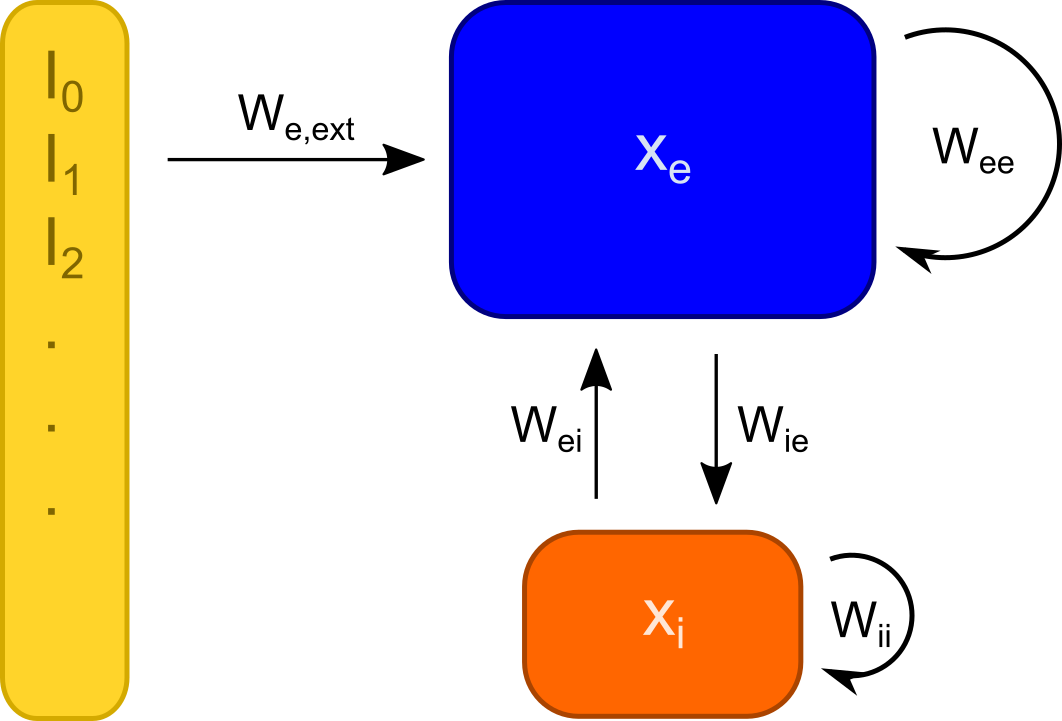
\includegraphics[width=0.7\textwidth]{../../plots/illustration.png}
\caption{\label{fig:architecture} Architecture of the RNN}
\end{figure}

The recurrent network consists of a population with $N_e = 300$ excitatory units (denoted as $x_e$) and a population with $N_i = 60$ (denoted as $x_i$) inhibitory units. Furthermore, a population of $N_{ext} = 9$ excitatory units ($I_j$) is interpreted as external input, where the input coming from each external unit is to be interpreted as encoding a particular feature of a sensory stream, e.g. the recognition of a particular letter or symbol.

\section{Methods} \label{Methods}
\subsection{Network Details}

Synaptic connectivities - represented by arrows in the illustration - were initially generated from a uniform distribution and the following properties, listed in Table \ref{tab:network_params}.

\begin{table}
\caption{Network parameters}
\begin{tabular}{l|r}
Connection Fraction $W_{ee}$ & $0.05$ \\
Connection Fraction $W_{ei}$ & $0.1$ \\
Connection Fraction $W_{ie}$ & $0.2$ \\
Connection Fraction $W_{ii}$ & $0.2$ \\
Connection Fraction $W_{e,ext}$ & $0.1$ \\
$\langle W_{e,ext} \rangle$ & $0.2$ \\
Total postsynaptic E$\rightarrow$E input & $1.0$ \\
Total postsynaptic I$\rightarrow$E input & $-1.0$ \\
Total postsynaptic E$\rightarrow$I input & $1.0$ \\
Total postsynaptic I$\rightarrow$I input & $-1.0$
\end{tabular}
\label{tab:network_params}
\end{table}


\subsection{Neuron Model}

The state of the neurons is updated in discrete time steps by the following equations:

\begin{align}
x_{e,n}(t+1) &= \theta\left( \sum_{j=0}^{N_e - 1} W_{ee,nj} x_{e,j}(t) + \sum_{k=0}^{N_i-1} W_{ei,nk} x_{i,k}(t)  + \sum_{l=0}^{N_{ext}-1} W_{e,ext,nl} I_{l}(t) - T_{e,n}(t) + \xi_{e,n}(t) \right) \label{eq:x_e_update} \\
x_{i,n}(t+1) &= \theta\left( \sum_{j=0}^{N_e - 1} W_{ie,nj} x_{e,j}(t) + \sum_{k=0}^{N_i-1} W_{ii,nk} x_{i,k}(t)  - T_{i,n}(t)  + \xi_{i,n}(t)\right) \label{eq:x_e_update}
\end{align}

where $\theta(\cdot)$ is the theta function and $T_e$ and $T_i$ represent additional threshold values. $\xi_{e/i}$ are random noise terms sampled from a Gaussian distribution at each time step with parameters $\mu_{noise,e/i}$ and $\sigma_{noise,e/i}$.

To stabilize network activity, each neuron's threshold is updated each time step such that the neuron's average activity approach a given target value:

\begin{equation}
T_{e/i,n}(t+1) = T_{e/i,n}(t) + \mu_{IP}\left(x_{e/i,n}(t)-r_{target,e/i,n}\right)
\end{equation}

where $\mu_{IP}$ is the learning rate of this ``intrinsic plasticity". Target rates $r_{target,e/i}$ were drawn randomly from a Gaussian distribution with parameters $\mu_{target,e/i}$ and $\sigma_{target,e/i}$ for each neuron and kept fixed throughout the simulation.

Parameters of the dynamics described in this section are given in Table \ref{tab:neuron_params}.
\begin{table}
\caption{Parameters of the neuron model}
\begin{tabular}{ll}
$\mu_{noise,e}$ & $0.0$ \\
$\mu_{noise,i}$ & $0.0$ \\
$\sigma_{noise,e}$ & $0.1$ \\
$\sigma_{noise,i}$ & $0.1$ \\
$\mu_{target,e}$ & $0.1$ \\
$\mu_{target,i}$ & $0.1$ \\
$\sigma_{target,e}$ & $0.0$ \\
$\sigma_{target,i}$ & $0.0$ \\
$\mu_{IP}$ & $0.002$
\end{tabular}
\label{tab:neuron_params}
\end{table}


\begin{comment}
<!--
w_mean_pre_ext_input = .2

w_exc_min = 0.0001
w_inh_max = -0.0001
##

## Neuron
g_neur = 20. # gain factor of the activation function

r_target_e_mu = 0.1 # mean homeostatic excitatory target firing rate
r_target_e_sigm = 0.#2 # standard deviation of homeostatic excitatory target firing rate
r_target_set_e = np.minimum(1.,np.maximum(0.,np.random.normal(r_target_e_mu,r_target_e_sigm,N_e)))

r_target_i_mu = 0.1 # mean homeostatic inhibitory target firing rate
r_target_i_sigm = 0.#2 # standard deviation of homeostatic inhibitory target firing rate
r_target_set_i = np.minimum(1.,np.maximum(0.,np.random.normal(r_target_i_mu,r_target_i_sigm,N_i))) 

mu_IP = 0.002 # threshold adaption rate

T_e_max_init = 1.
T_i_max_init = 1.

mu_mem_noise = 0.
sigm_mem_noise = np.sqrt(0.01)
##

## Synaptic Normalization
w_total_ee = .5#*N_e**.5 # total presynaptic E->E input
#w_total_eext = .5 # total presynaptic Ext->E input
w_total_ei = -1.#*N_i**.5 # total presynaptic I->E input
w_total_ie = 1.#*N_e**.5 # total presynaptic E->I input
w_total_ii = -1.#*N_i**.5 # total presynaptic I->I input
##
\end{comment}

\subsection{Rules of the Input Sequence}

In each time step, only a single unit is in its active state $I_j(t) = 1$. The sequence of active input nodes was generated by a markov chain with transition probabilities shown in Fig. \ref{fig:grammar_markov}.

\begin{figure}
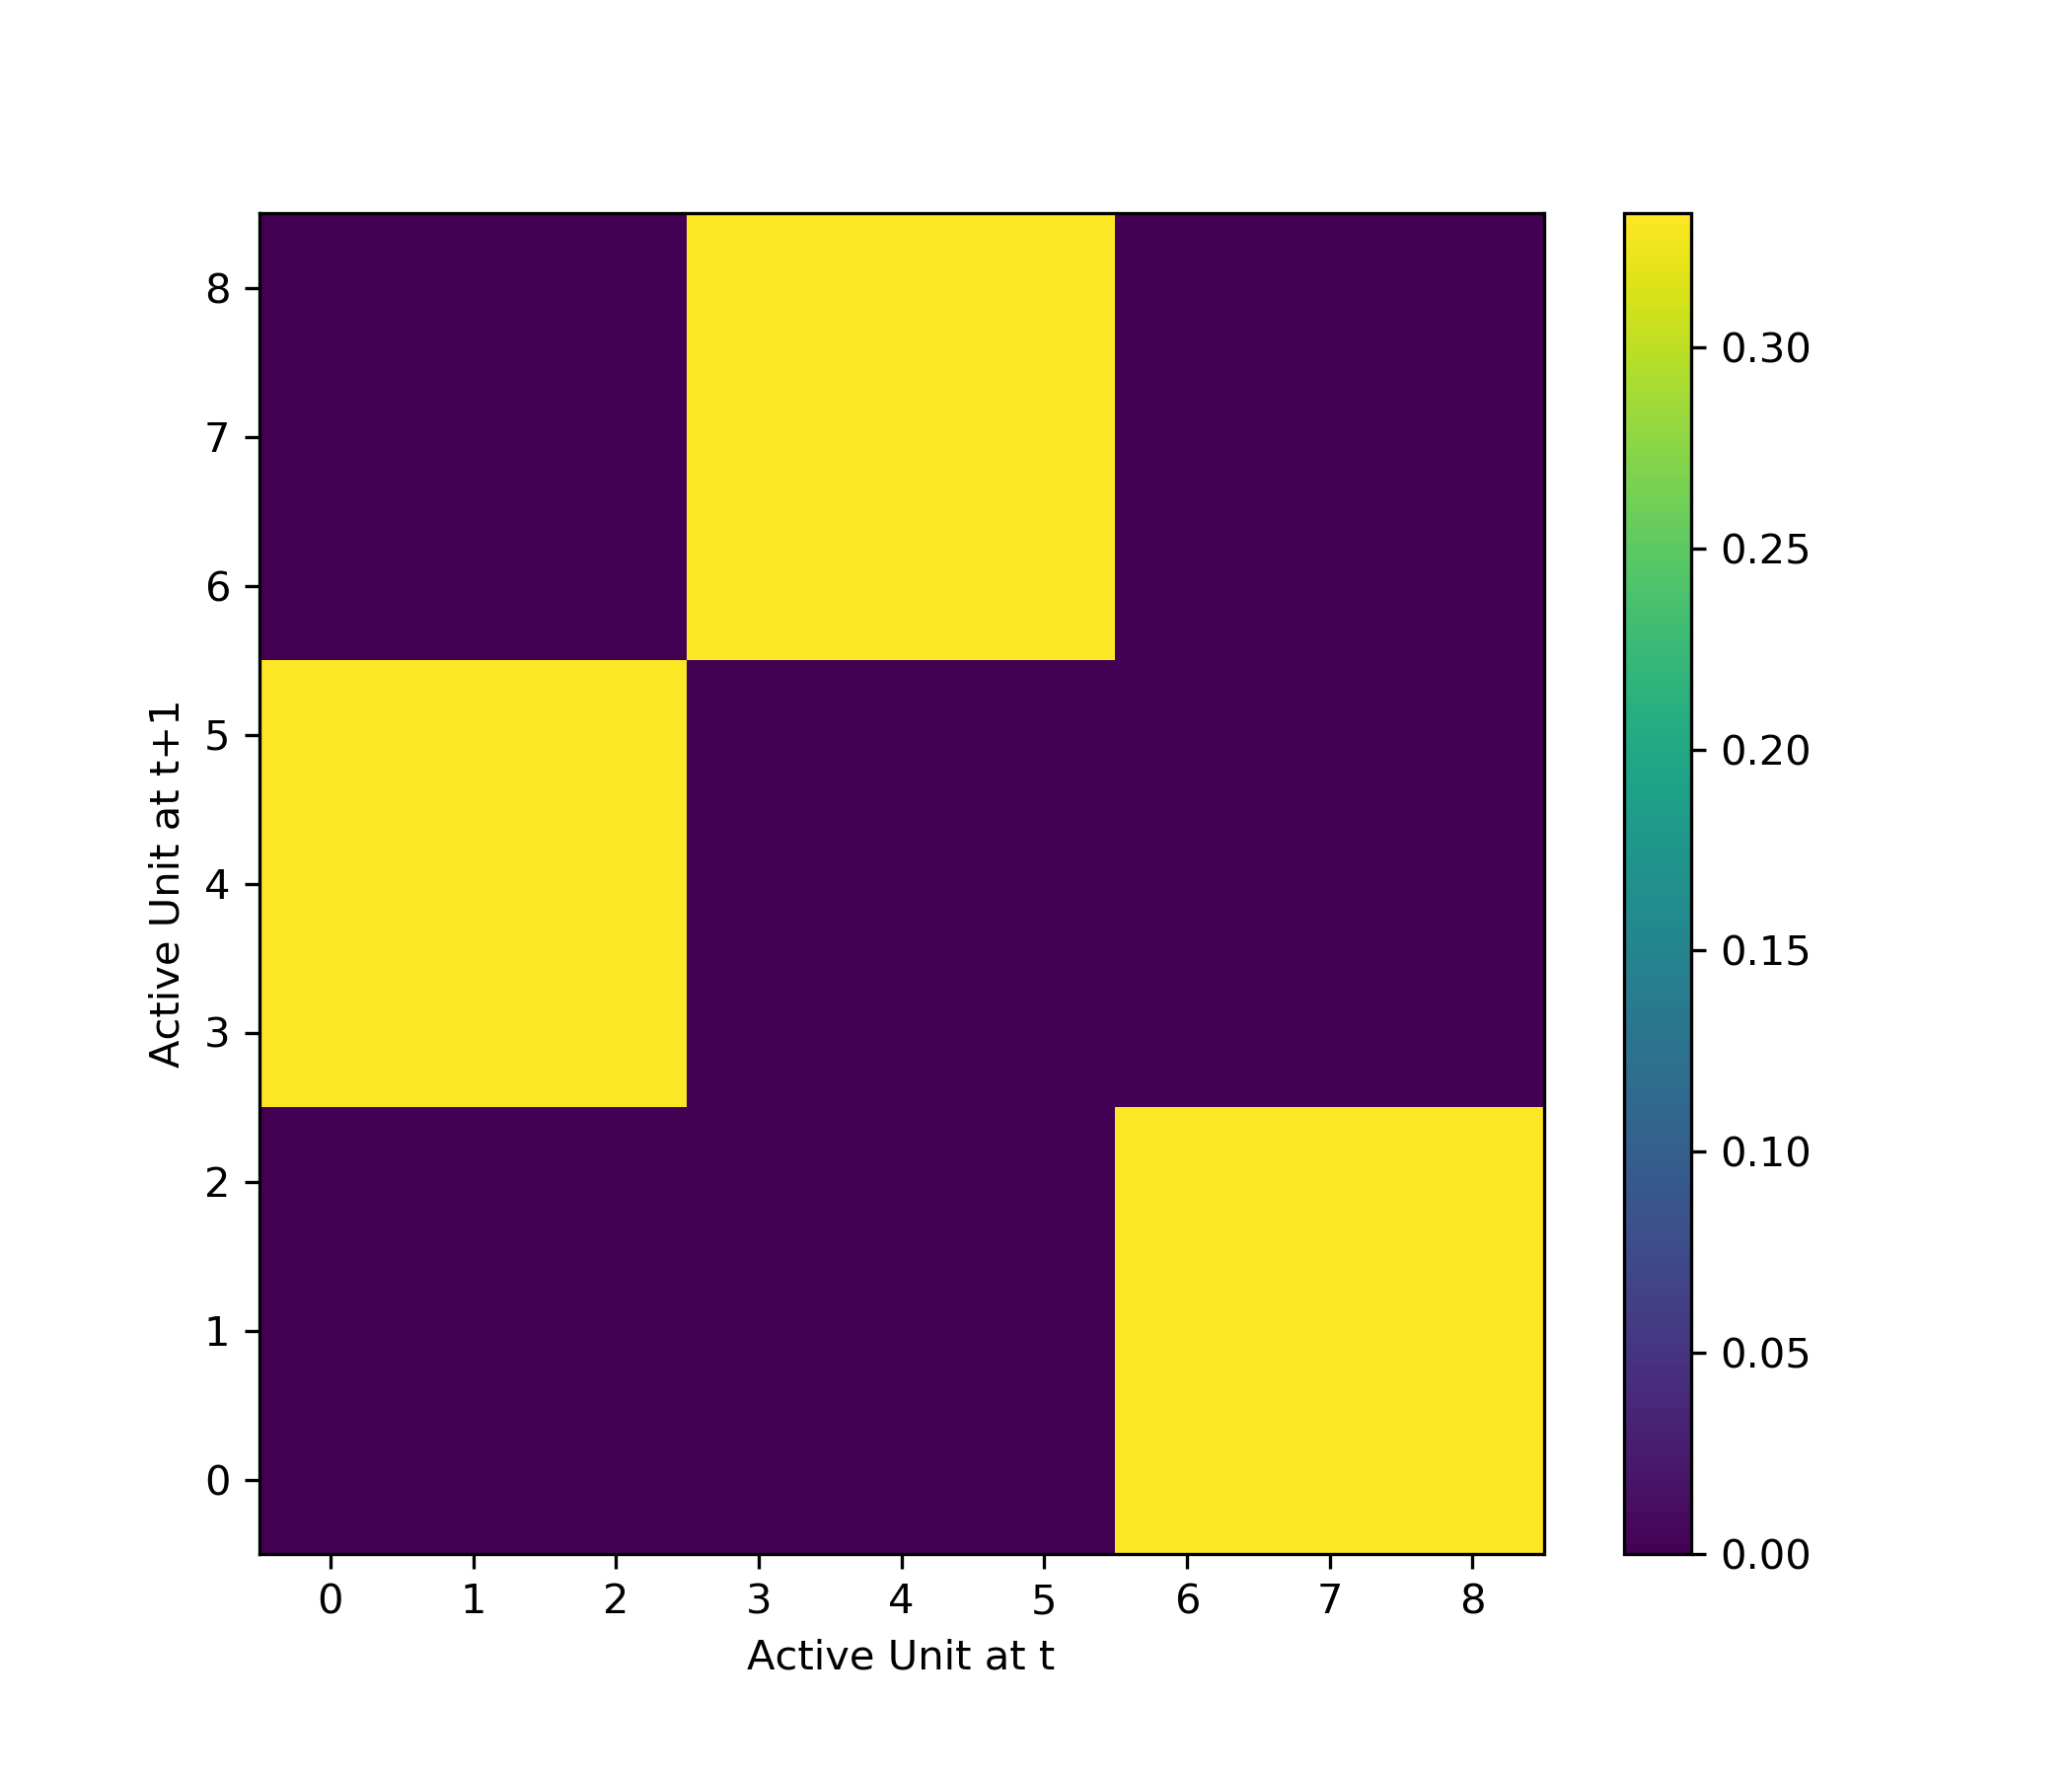
\includegraphics[width=\textwidth]{../../plots/Grammar_Markov.png}
\caption{\label{fig:grammar_markov} Transition Matrix between subsequently active input states}
\end{figure}

Due to the structure of the transition matrix, the sequence is partially predictable in the sense that an element of $\{0,1,2\}$ will always be followed by an element of $\{3,4,5\}$ etc.

\subsection{Plasticity Rules}

Recurrent excitatory connection were subject to two plasticity mechanisms: A simple pre-post Hebbian learning rule and a postsynaptic multiplicative normalization preventing connectivity runaway.

\begin{align}
\Delta W_{ee,ij}(t) &= \mu_{hebb} \left( x_{e,j}(t-1)x_{e,i}(t) - x_{e,i}(t-1)x_{e,j}(t) \right) \\
W_{ee,ij}(t) &= w_{total,ee}\frac{W_{ee,ij}(t-1) + \Delta W_{ee,ij}(t)}{\sum_{k=0}^{N_e - 1} W_{ee,ik}(t-1) + \Delta W_{ee,ik}(t)}
\end{align}

We did not include pruning or creation of synapses, but set a very small lower bound for existing excitatory connections.

\section{Results}

Network activity settled at a constant mean rate and a corresponding mean treshold, see Fig. \ref{fig:pop_act_time} and Fig. \ref{fig:thresholds_time}. 

\begin{figure}
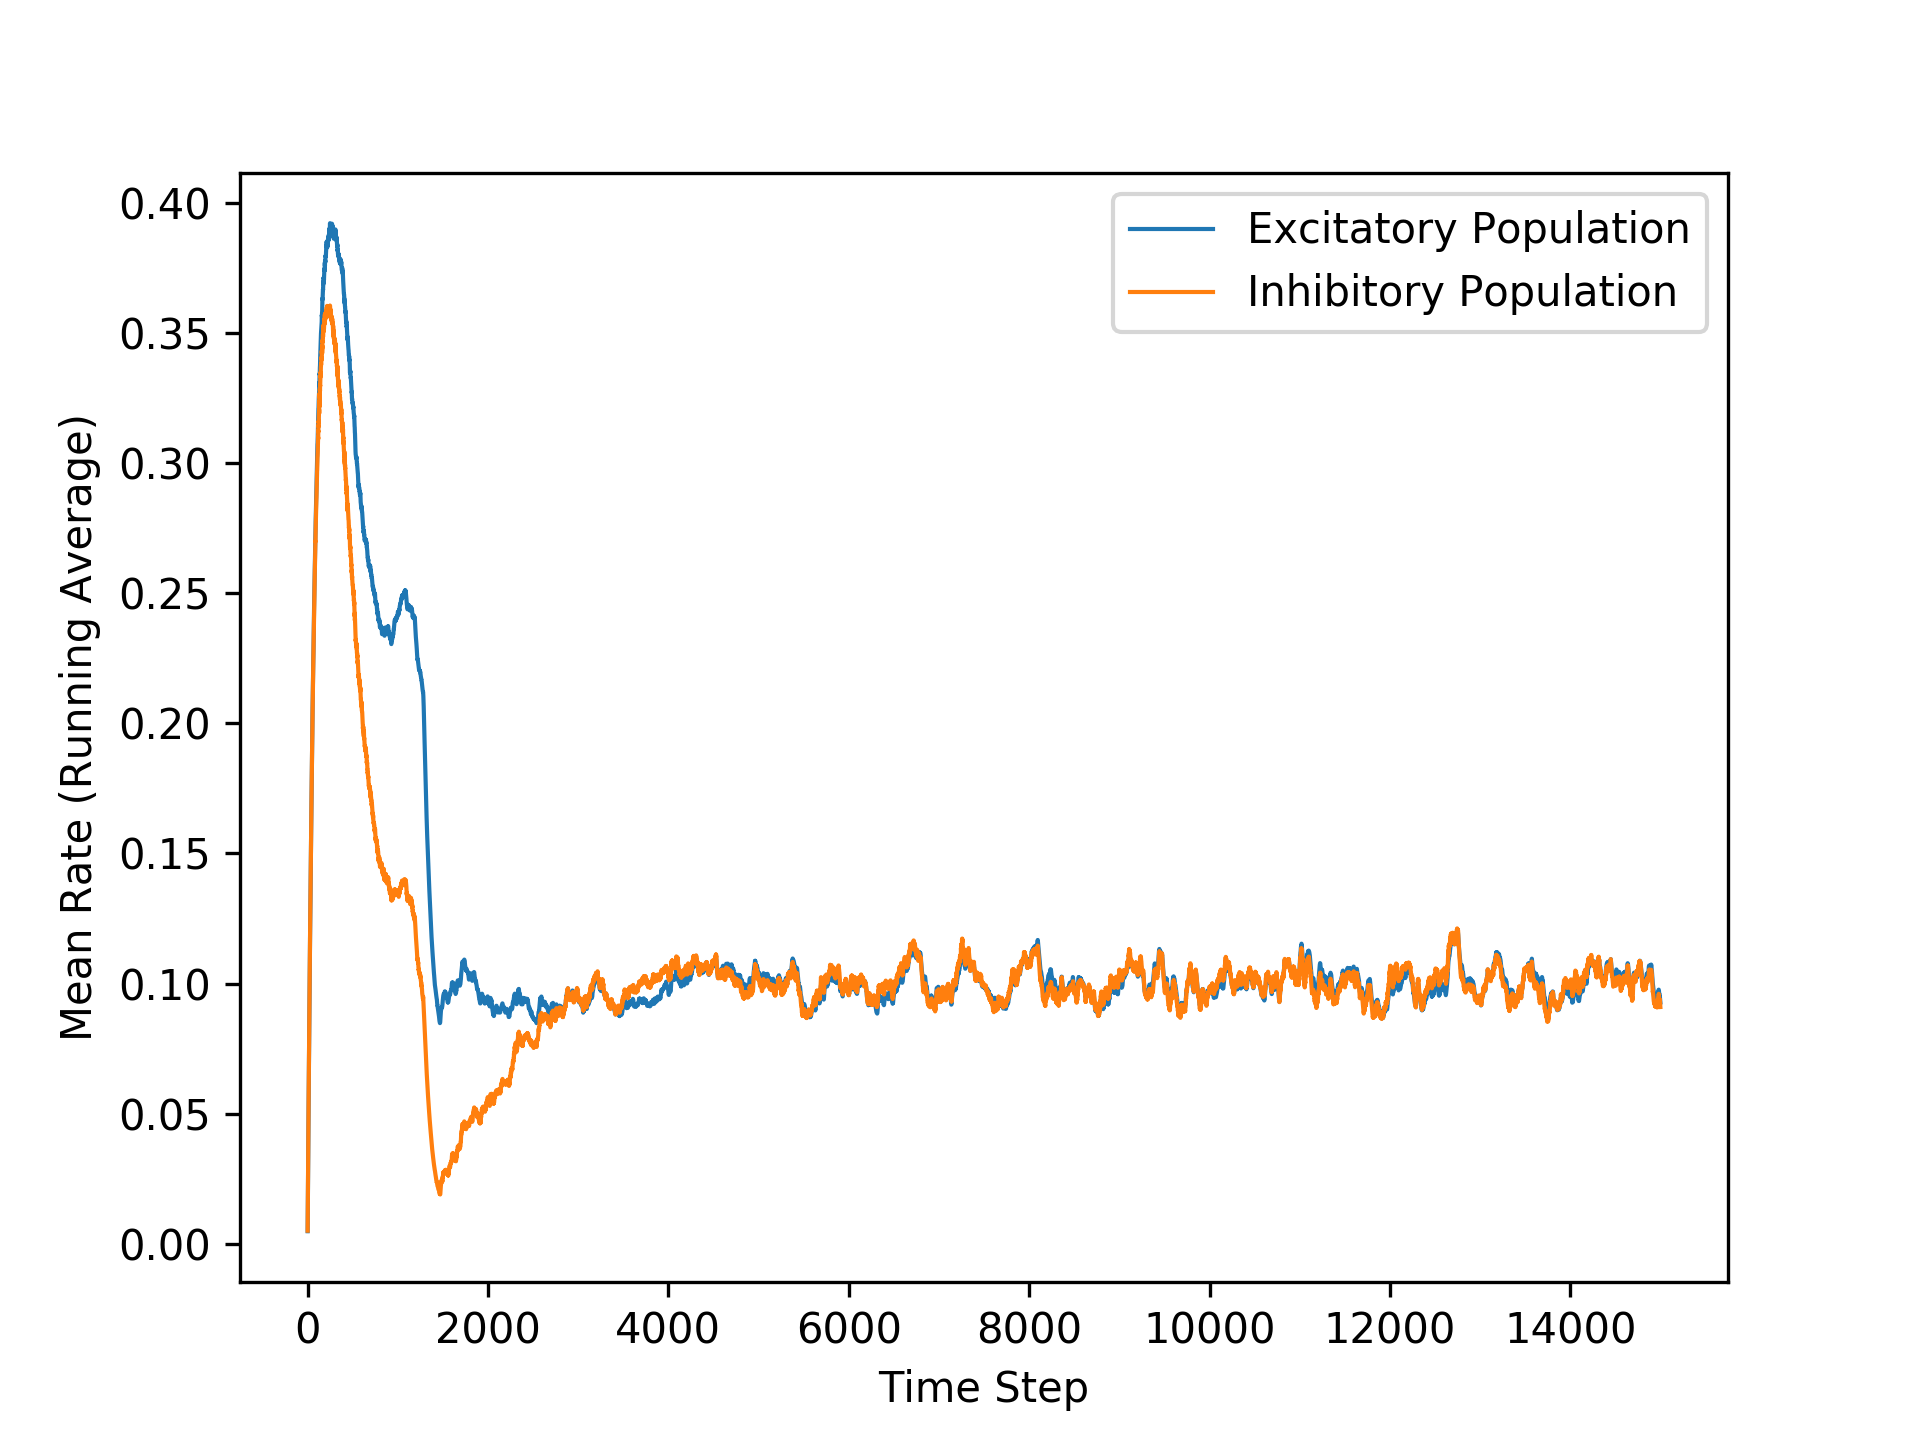
\includegraphics[width=\textwidth]{../../plots/pop_act_time.png}
\caption{\label{fig:pop_act_time} Running average of excitatory and inhibitory population activity.}
\end{figure}

\begin{figure}
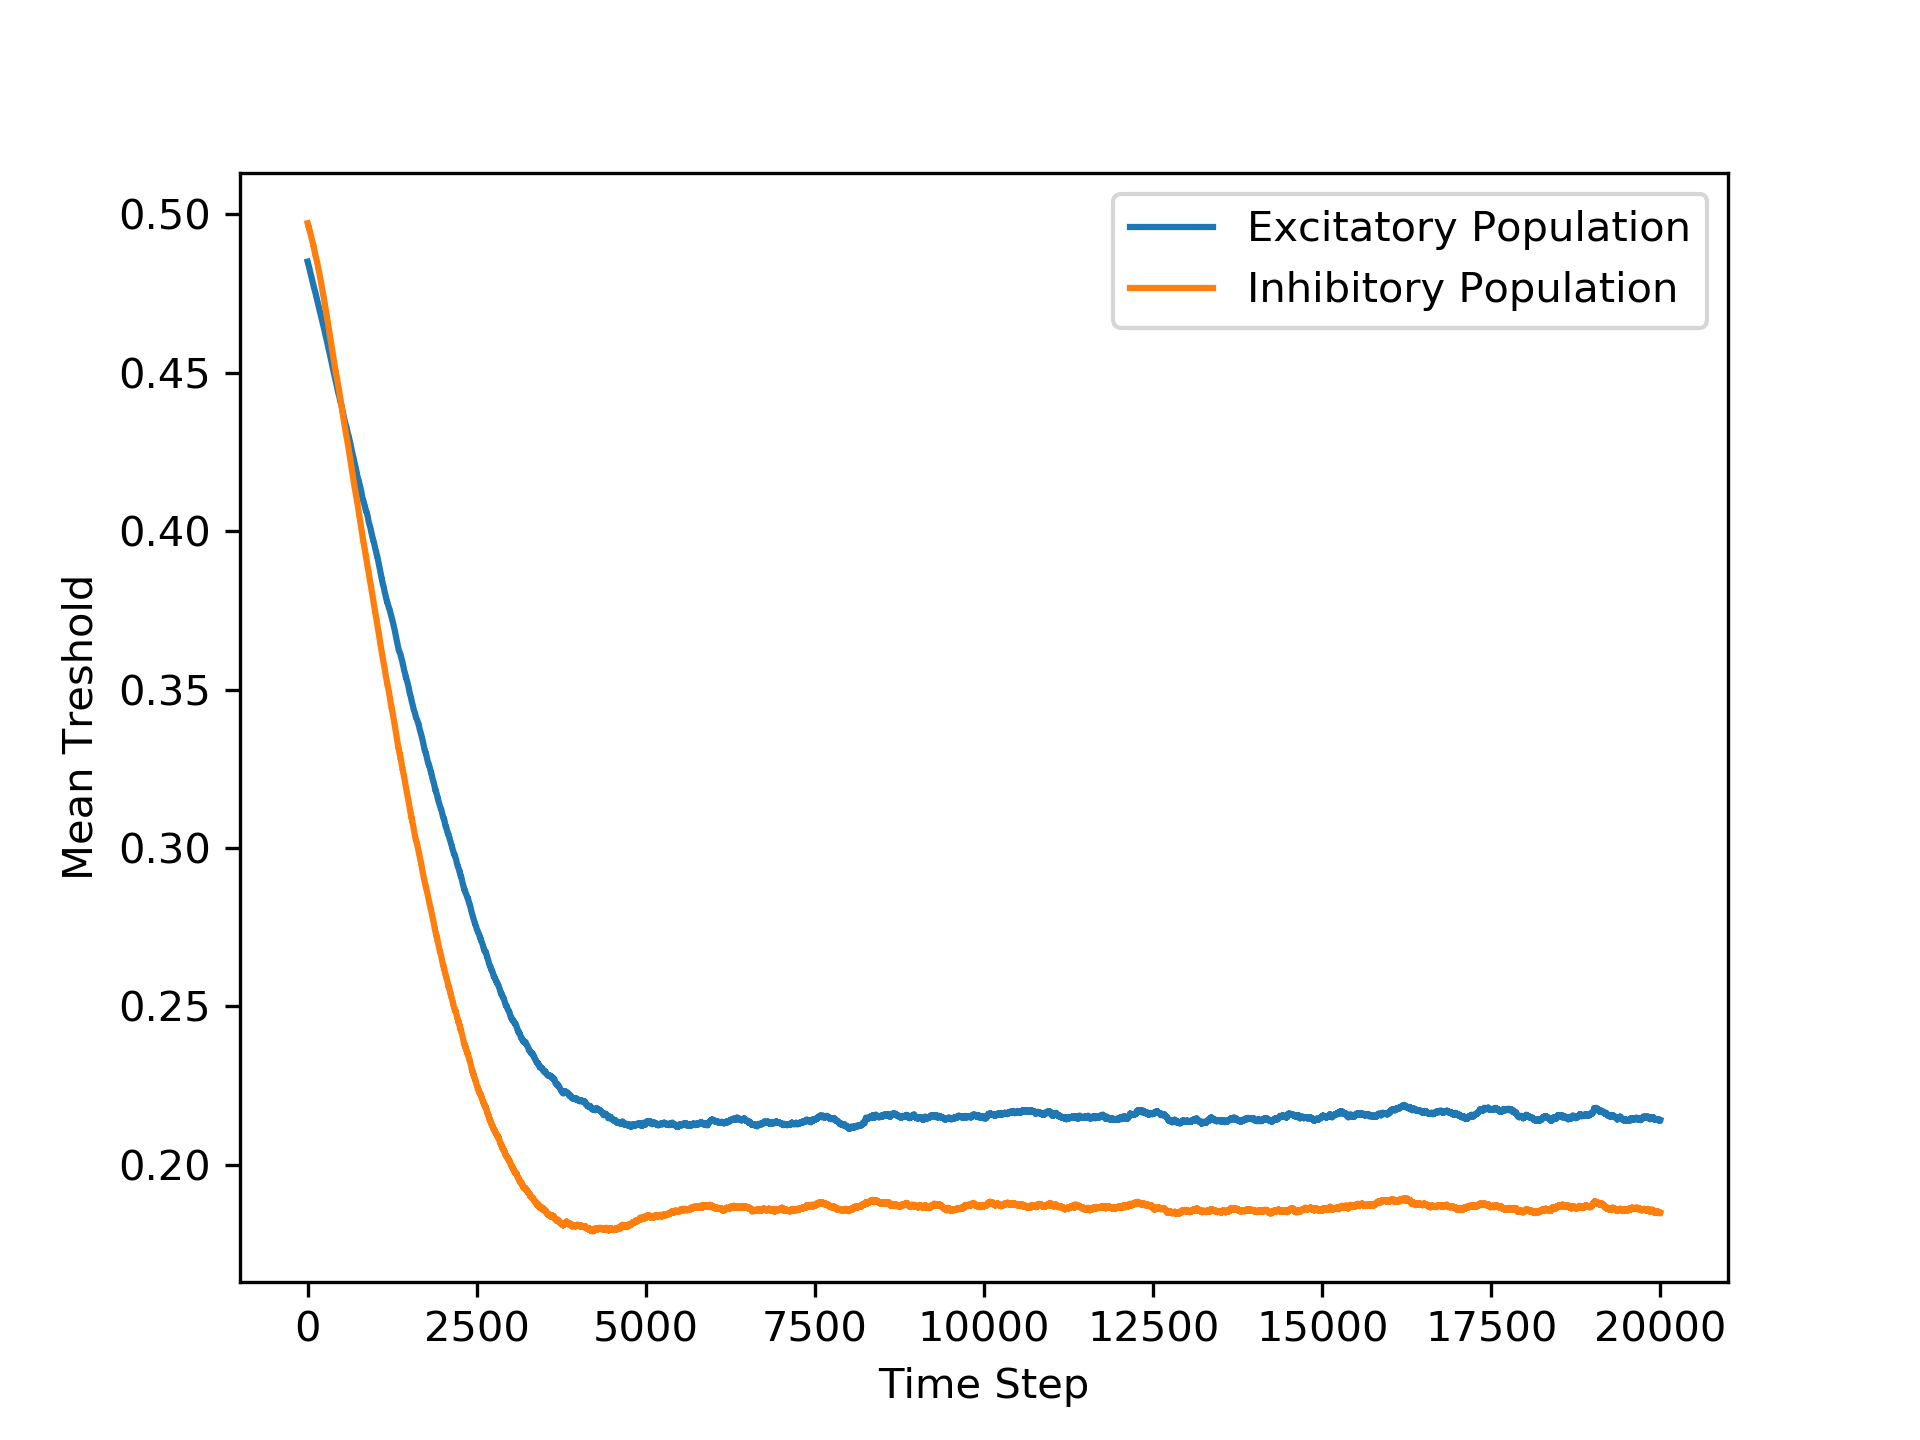
\includegraphics[width=\textwidth]{../../plots/thresholds_time.png}
\caption{\label{fig:thresholds_time} Population mean of excitatory and inhibitory thresholds.}
\end{figure}

Furthermore, Fig. \ref{fig:act_raster} and Fig. \ref{fig:isi_dist} suggest that the appearance of active states follows poissonian statistics. However, the distribution of excitatory inter``spike"-intervals shows a clear preference for multiples of 3, which was not present in the absence of external input and is reflected in the 3-fold periodicity of the input sequence. 

\begin{figure}
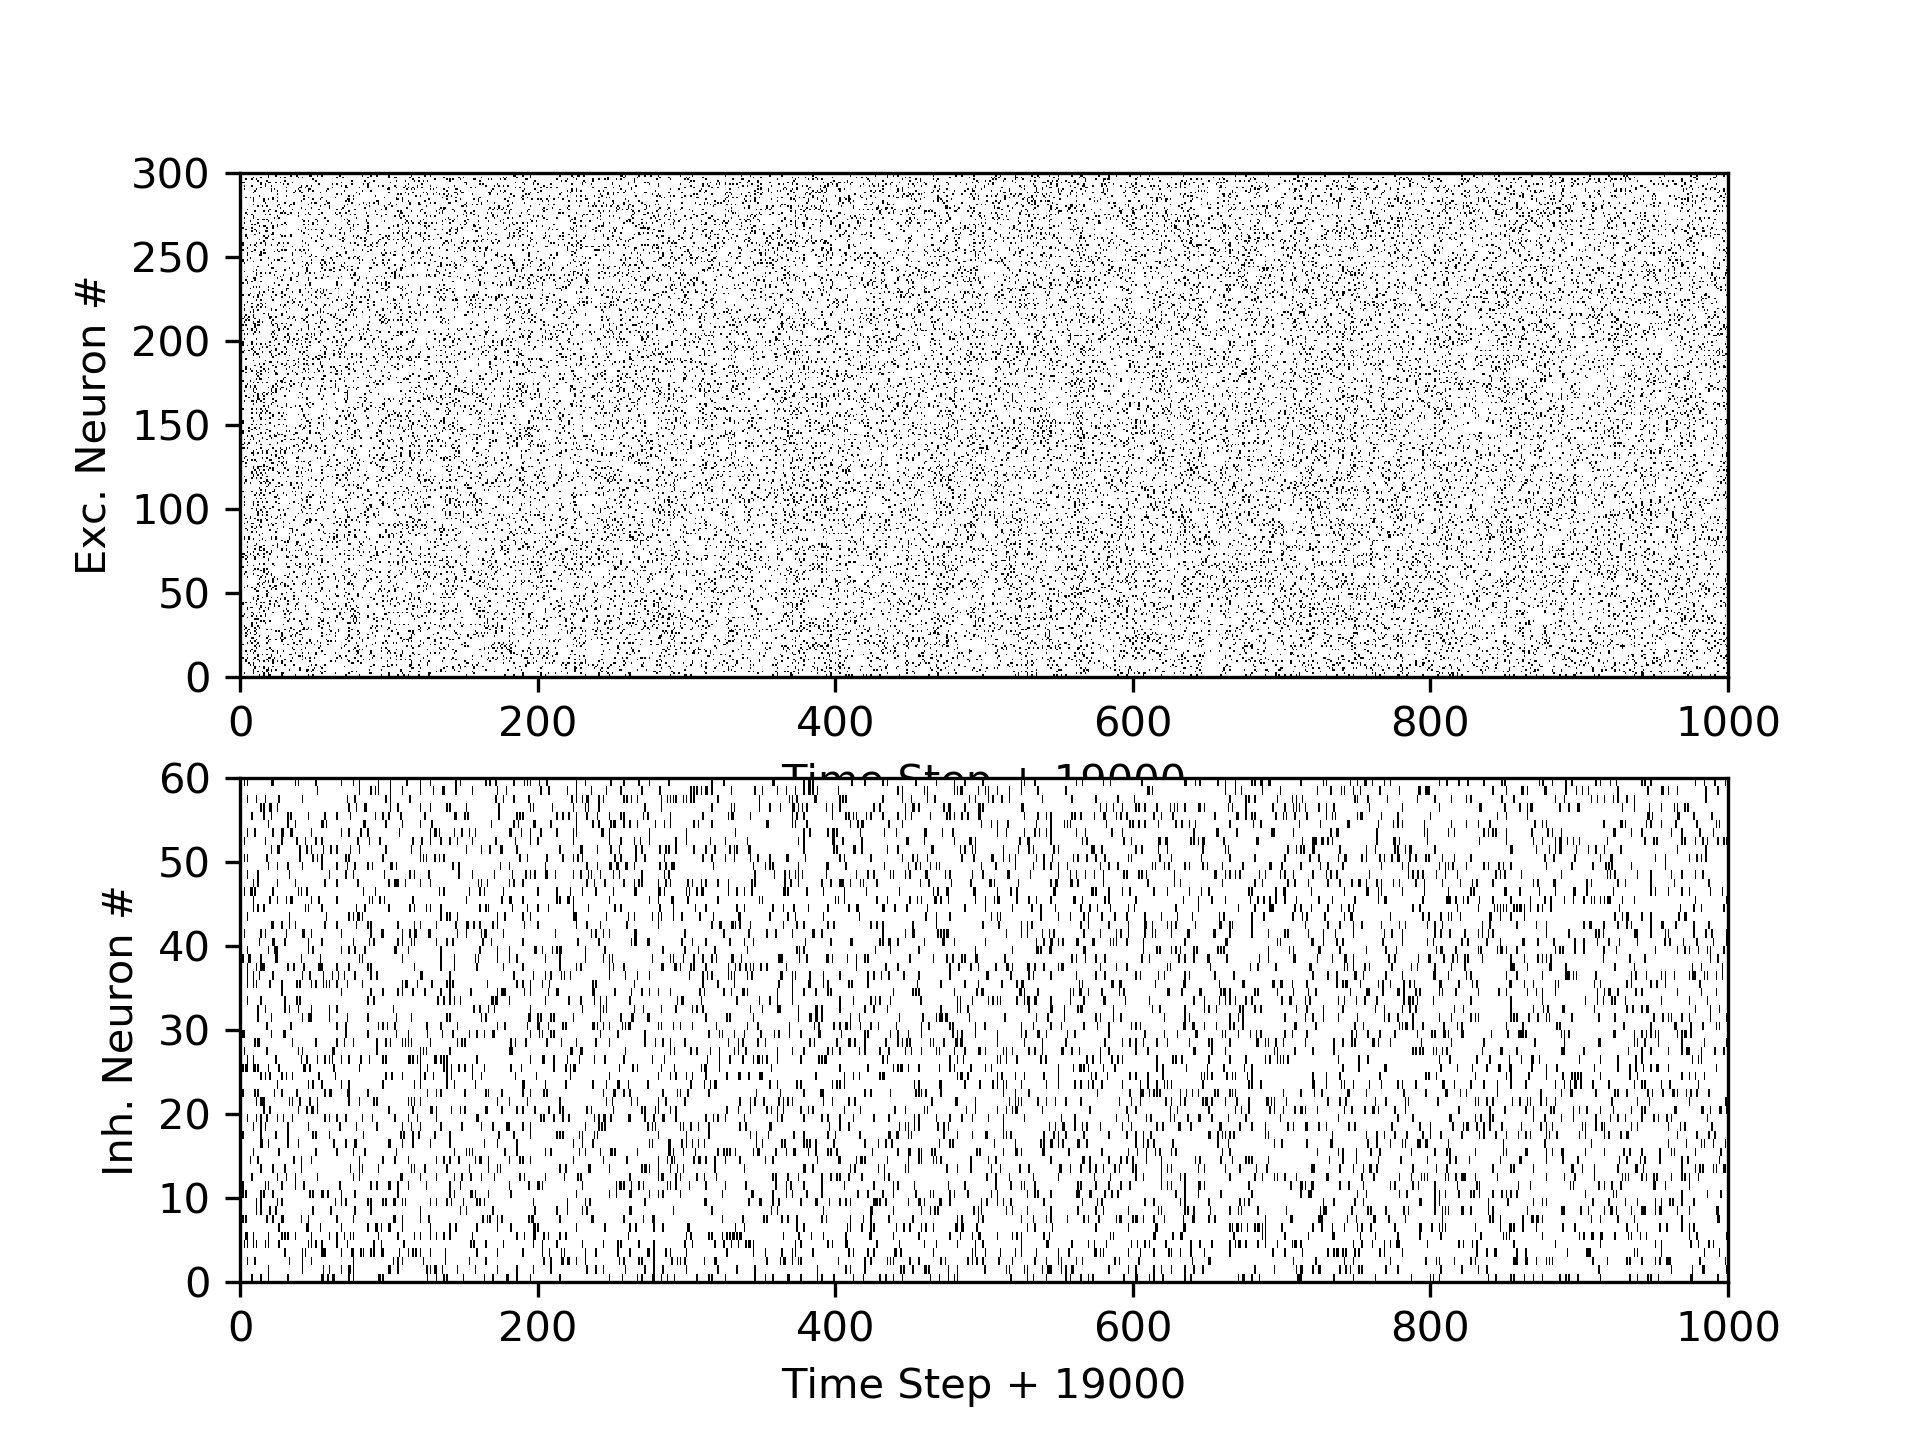
\includegraphics[width=\textwidth]{../../plots/act_raster.png}
\caption{\label{fig:act_raster} Raster plot of network activity.}
\end{figure}

\begin{figure}
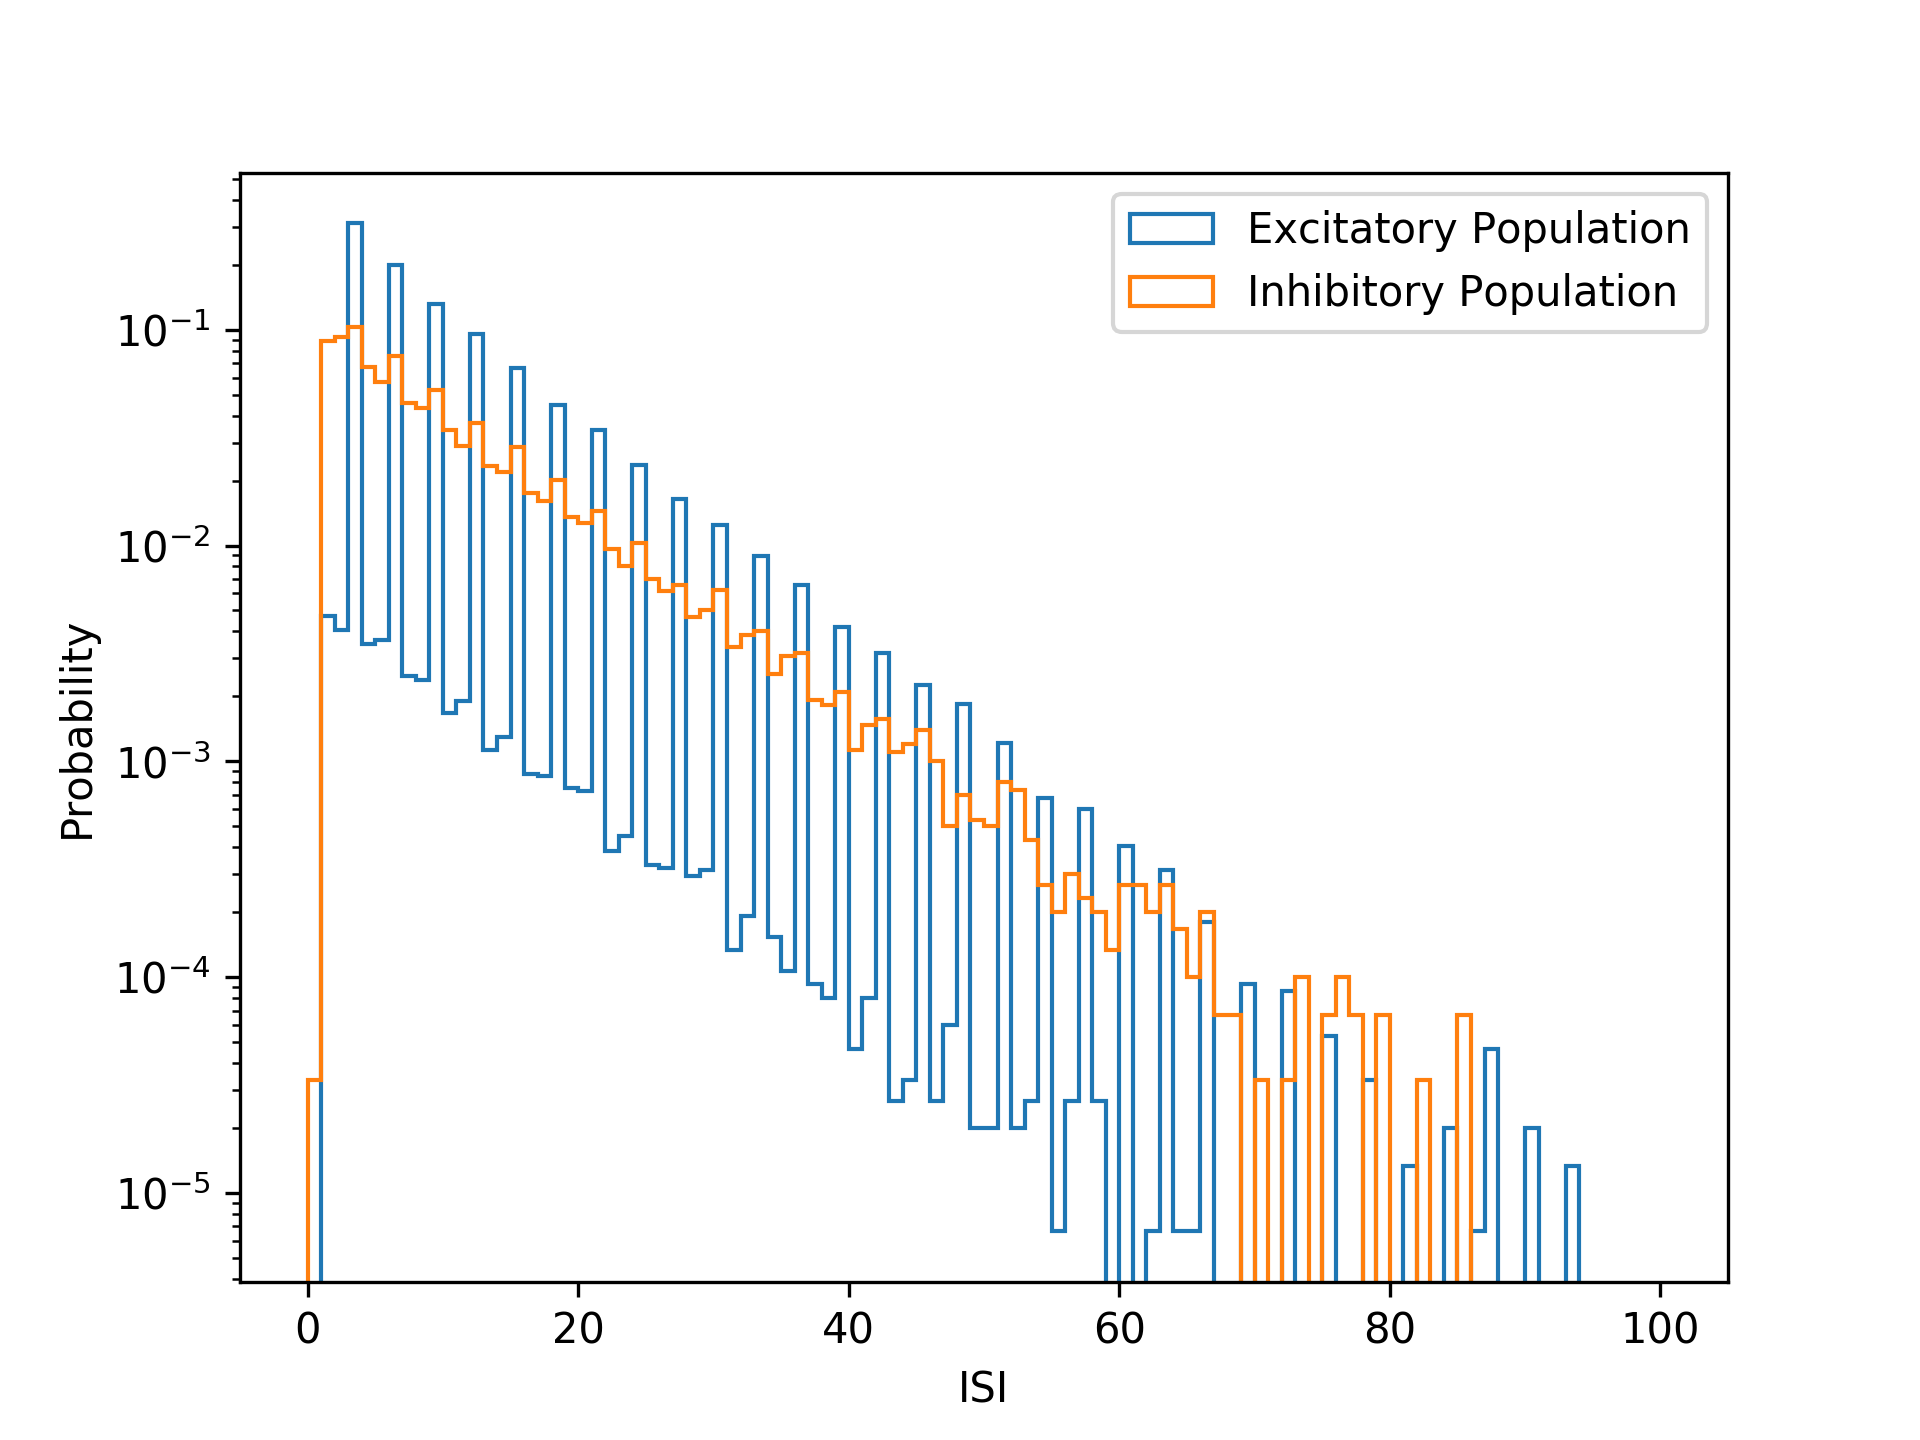
\includegraphics[width=\textwidth]{../../plots/isi_dist.png}
\caption{\label{fig:isi_dist} Distribution of interspike intervals.}
\end{figure}

Generally speaking, the implemented plasticity rules often gave rise to time courses of synaptic weights similar to the one shown in Fig. \ref{fig:w_ee_sample_time}: the emergence of one or more comparably strong weights alongside a majority of weak connections.

\begin{figure}
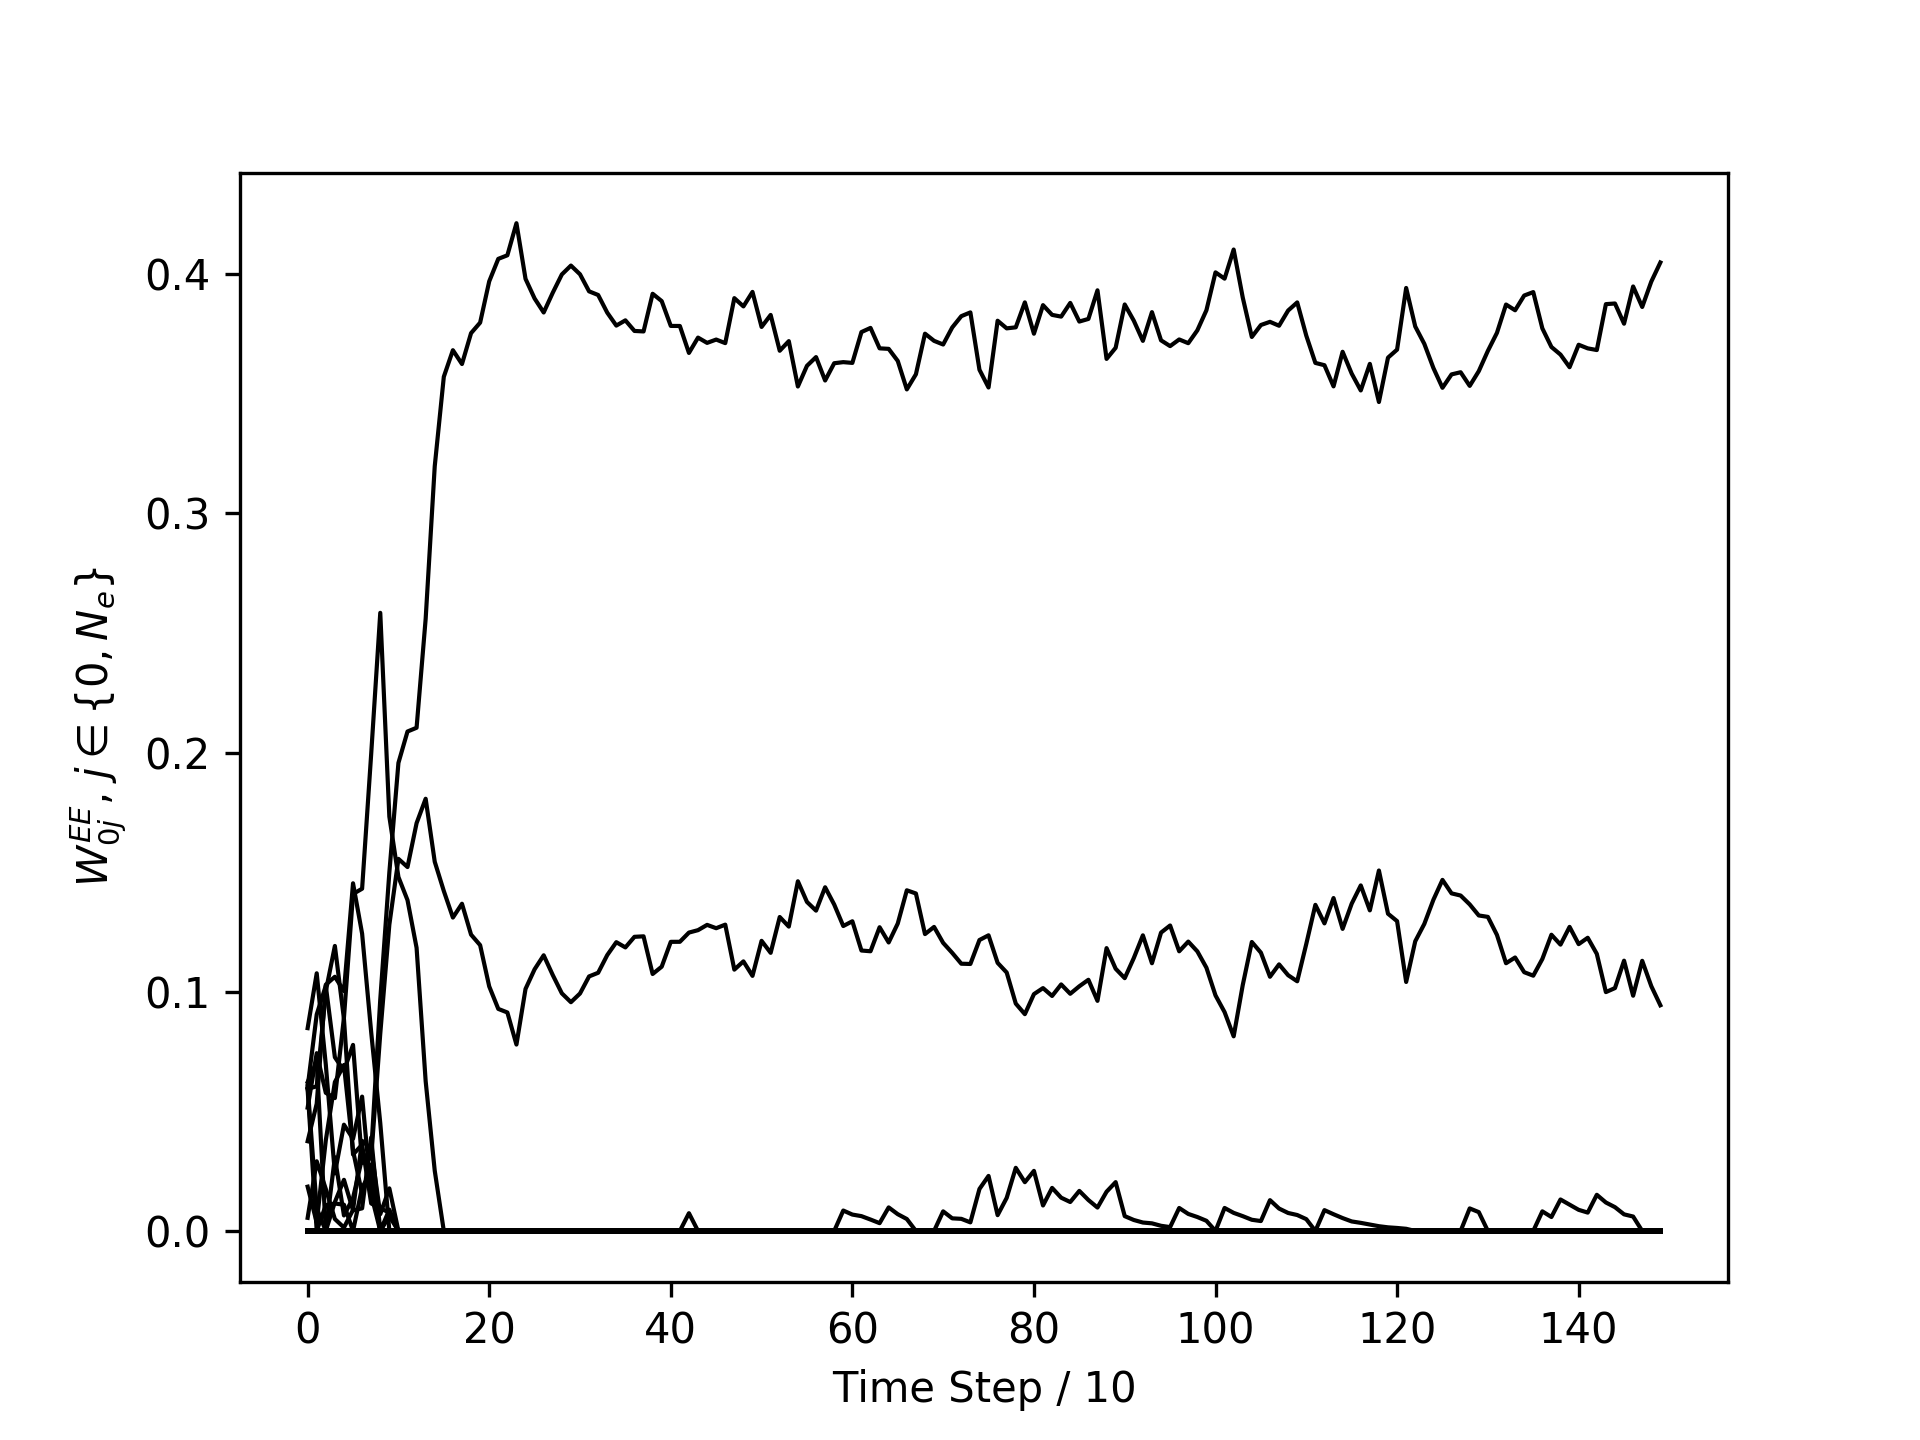
\includegraphics[width=\textwidth]{../../plots/w_ee_sample_time.png}
\caption{\label{fig:w_ee_sample_time} Sample time course of E->E weights.}
\end{figure}

\subsection{Cluster Analysis of Excitatory Activity}

Following the conceptual idea presented by Elman \cite{Elman_1990}, we performed a hierarchical cluster analysis of the binary activity vectors of the exitatory population. For this, we used the activity data of $x_e$ from the last $3000$  steps. We then performed a hierachical cluster analysis with Ward's method. The resulting dendrogram is depicted in Fig. \ref{fig:act_dendrogram}. A 3-fold structure is visible in the uppermost branching layer.

\begin{figure}
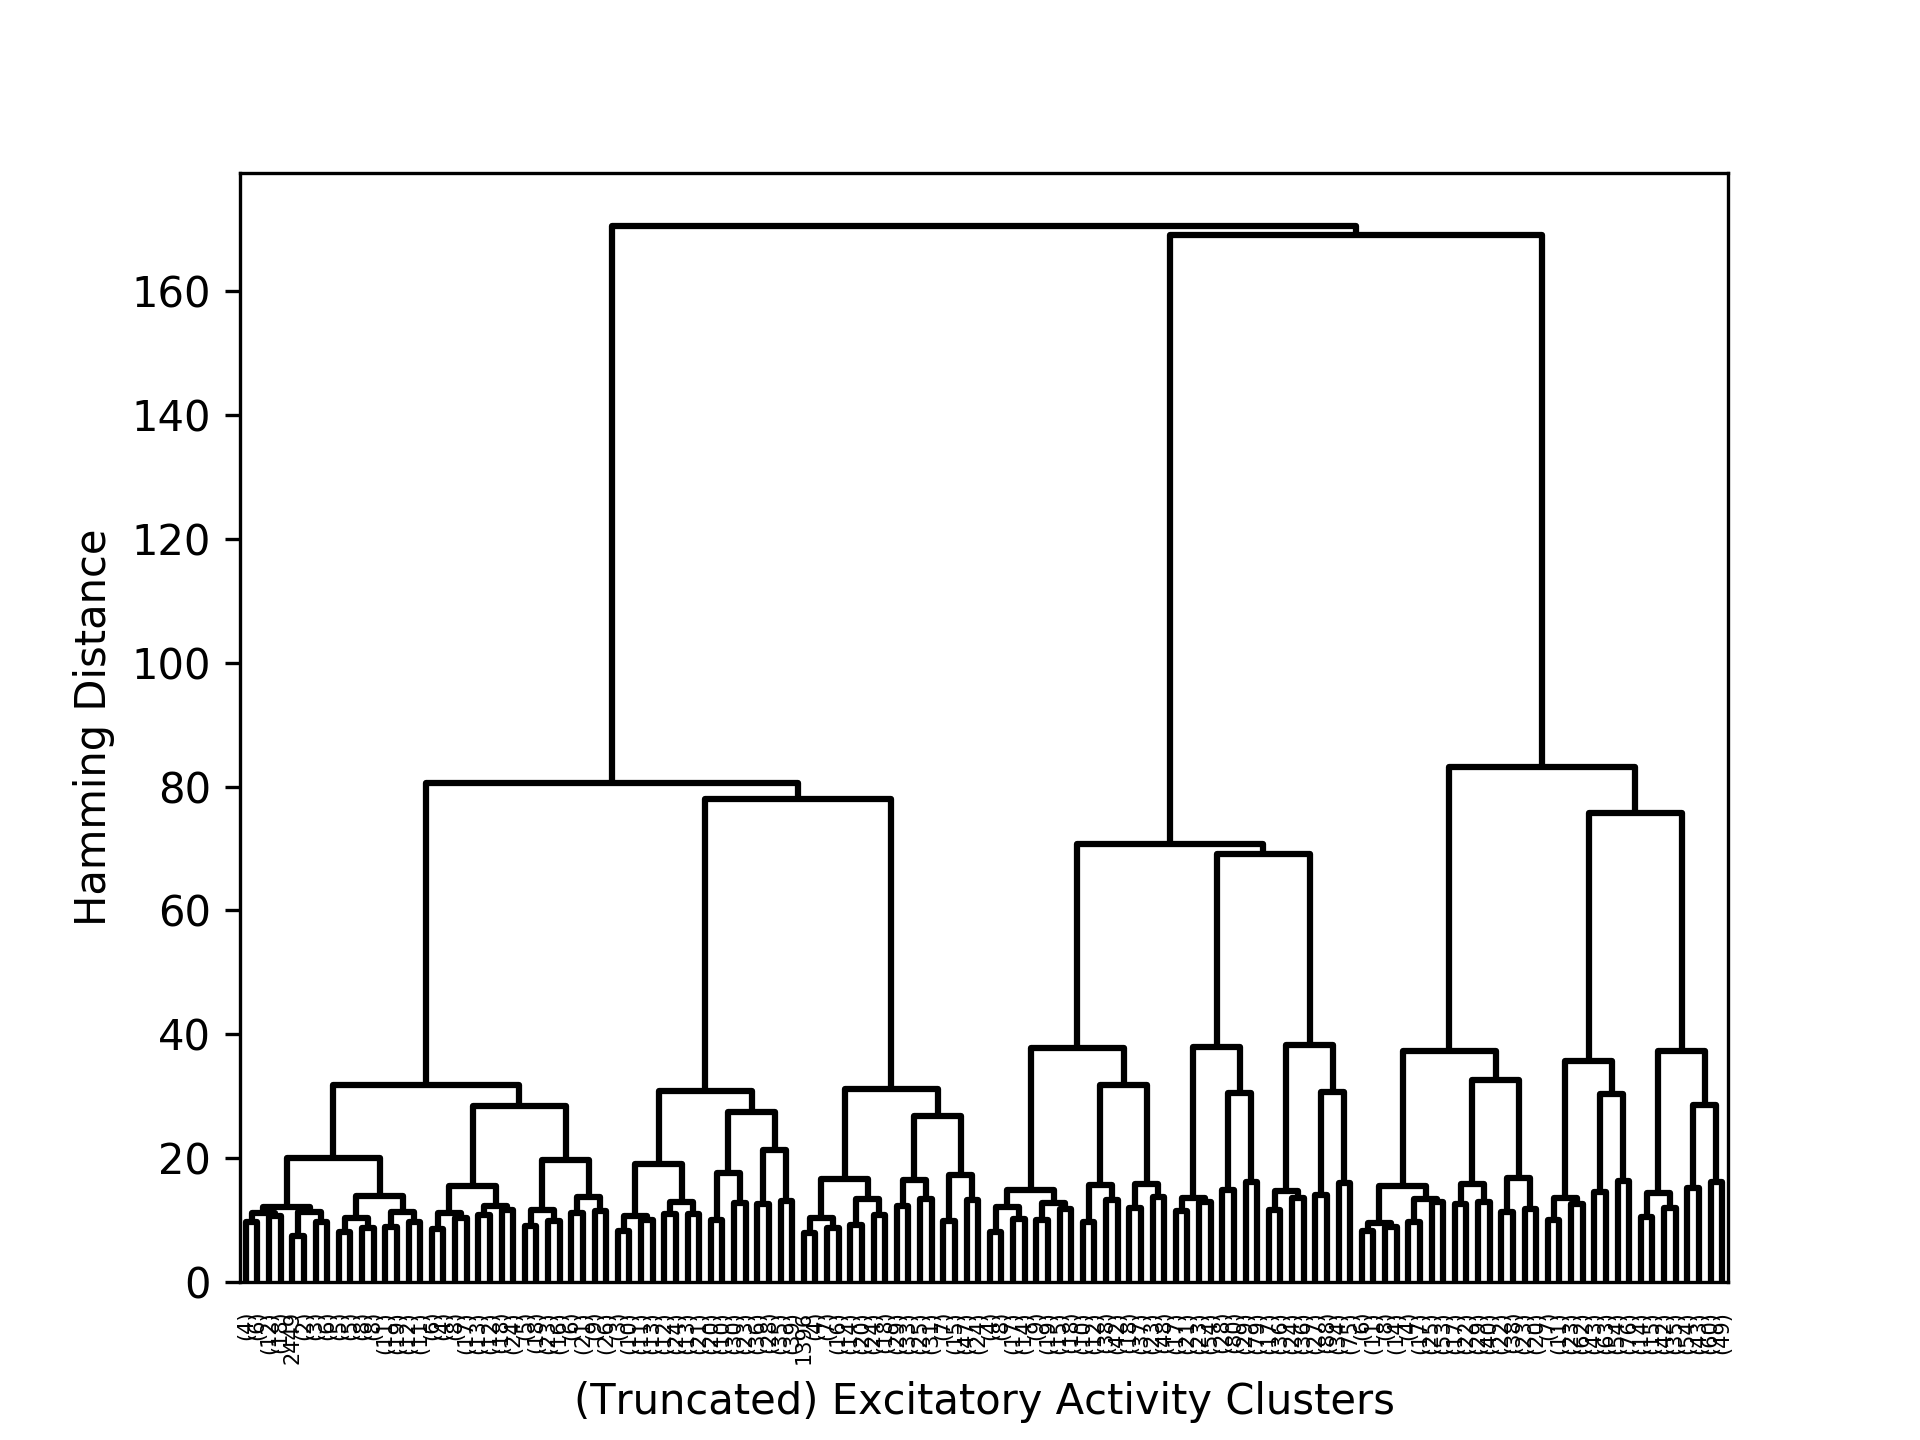
\includegraphics[width=\textwidth]{../../plots/act_dendrogram.png}
\caption{\label{fig:act_dendrogram} Dendrogram of a cluster analysis of excitatory activity patterns.}
\end{figure}

Furthermore, if we use the cluster analysis to reorder the recurrent weight matrix after the plasticity phase in such a way that units with correlated activity are listed next to each other, we observe a structure depicted in Fig. \ref{fig:corr_weight_mat}. In particular, the weight matrix resembles the structure of the transition matrix shown in Fig. \ref{fig:grammar_markov}.

\begin{figure}
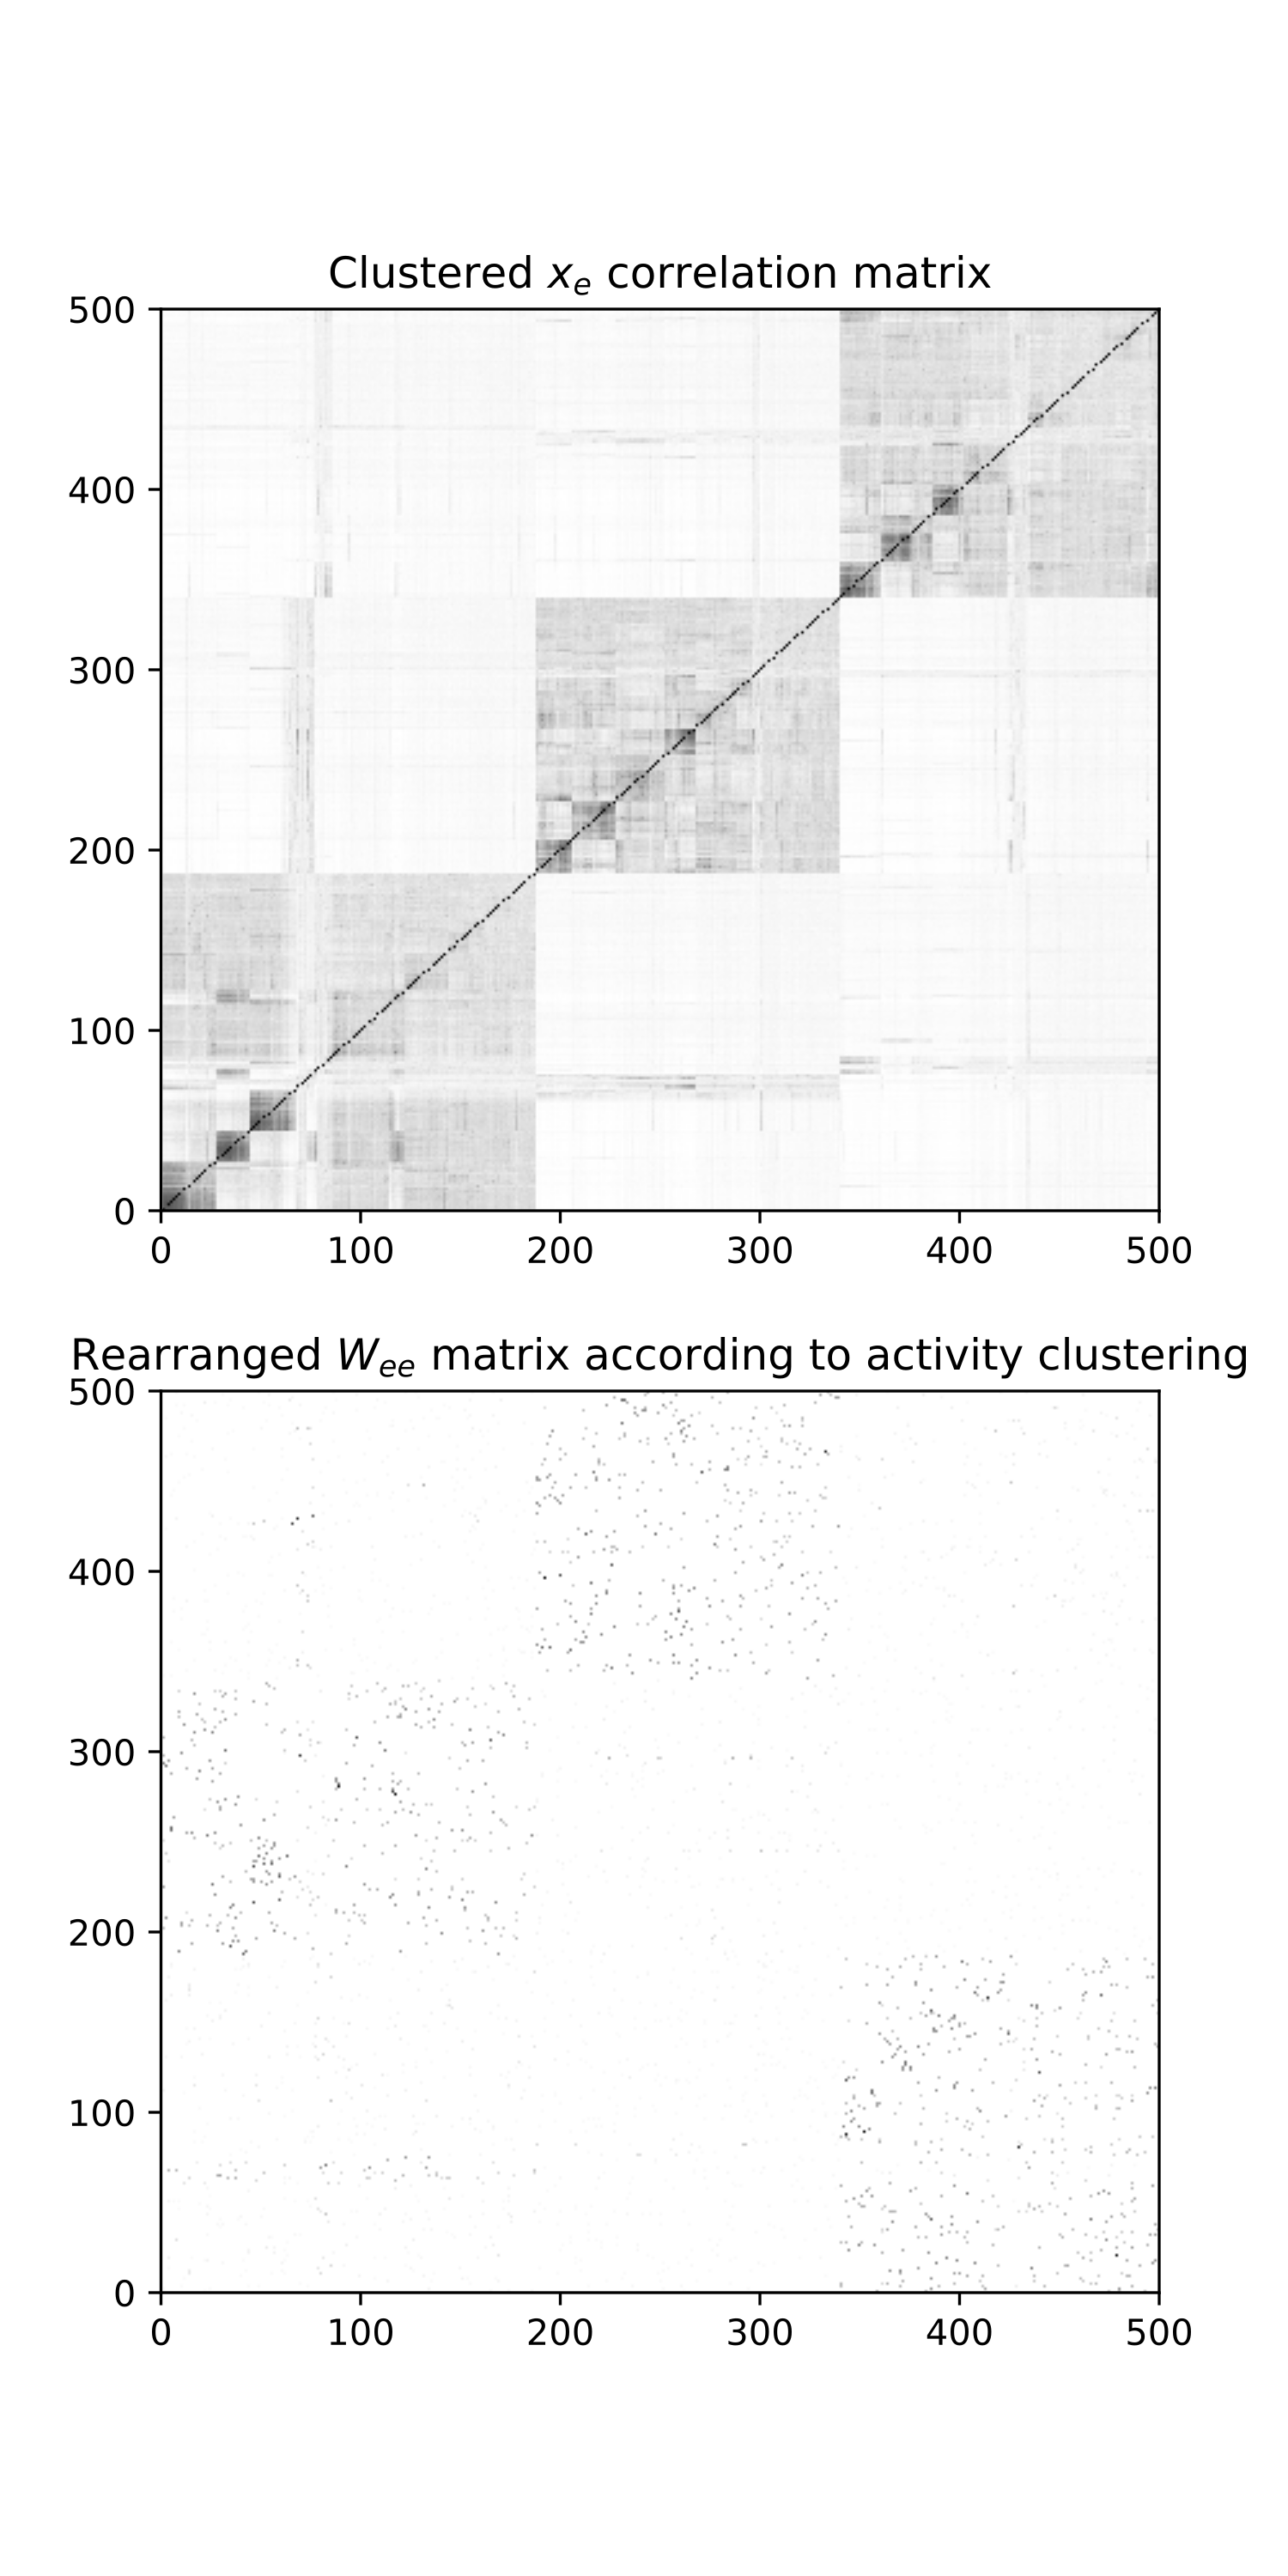
\includegraphics[width=0.8\textwidth]{../../plots/corr_weight_mat.png}
\caption{\label{fig:corr_weight_mat} Top: Correlation matrix of $x_e$ according to the clustering depicted in Fig. \ref{fig:act_dendrogram}. Bottom: Recurrent weight matrix after plasticity, ordered based on the same clustering.}
\end{figure}

\section{Using a Simple Model of Dendritic Separation}
So far, the neuron model we used was a simple point neuron model, which did not distinguish between input received by recurrent connection and the one stemming from recurrent connections. As such, one can argue that the emergence of a network structure reflecting the temporal structure of the external input significantly relies on the network being mostly driven by this external signal. Subpopulations subsequently being activated by the external input develop stronger connections due to the pre-post structure of the Hebbian plasticity rule. It is reasonable to assume that this ``driven learning" easily overrides any more complex structure that could potentially arise within the recurrent network.

Recently, nonlinear interactions between dendritic input proximal and distal to the soma have been investigated \cite{Shai_2015,Bono_2017}. Based on experimental findings and detailed neuronal compartment models, Shai et al. proposed a relatively simple phenomenological rate model that subsumes proximal and distal inputs into two input streams: Given some basal synaptic input $Y_p$ and distal input $Y_d$, we express the postsynaptic firing rate as
\begin{align}
M &= a_1 + a_2 \sigma \left( \left(Y_d-a_3\right) / a_4 \right) \label{f_comp1} \\ 
T &= b_1 + b_2 \sigma \left( \left(Y_d-b_3\right) / b_4 \right) \label{f_comp2}\\ 
f_{\rm comp} &= M \sigma \left(\left(Y_p - T \right) / c \right) \label{f_comp3}\\
\sigma (x) &= \frac{1}{1+\mathrm{exp}(-x)} \label{f_comp4}
\end{align}
where the parameters given in Table \ref{params_f_comp} were chosen to fit the composite function in \cite{Shai_2015}. Fig. \ref{fig:f_comp_plot} shows the resulting dependence on the input: maximum postsynaptic activity is only achieved with a combination of basal and proximal input. However, intermediate activity can also be observed by sufficient proximal input.
\begin{table}
\begin{center}
\caption{Parameters for \eqref{f_comp1} - \eqref{f_comp3}.}
\begin{tabular}{l|l}
$a_1$ & $0.5$ \\
$a_2$ & $0.5$ \\
$a_3$ & $0.36$ \\
$a_4$ & $0.05$ \\
$b_1$ & $0.1$ \\
$b_2$ & $0.5$ \\
$b_3$ & $0.3$ \\
$b_4$ & $-0.063$ \\
$c$ & $0.003$
\end{tabular}
\label{params_f_comp}
\end{center}
\end{table}

\begin{figure}
\centering
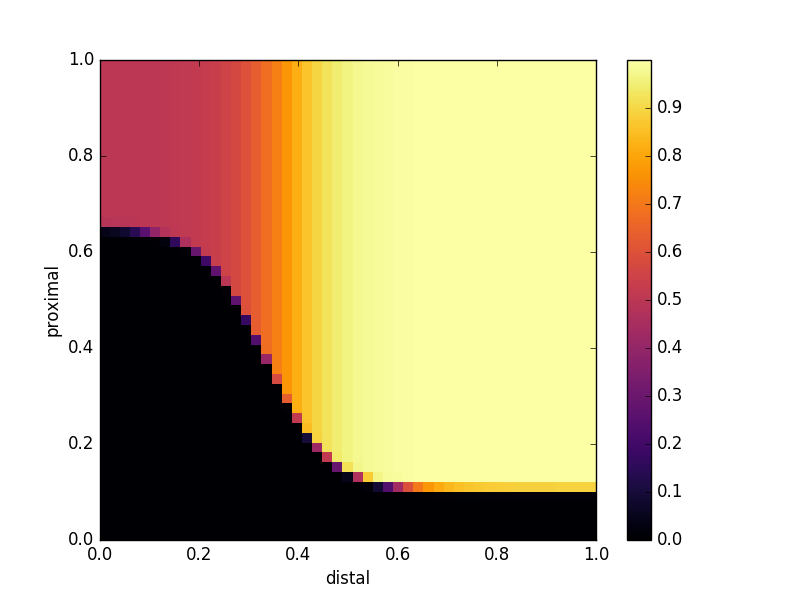
\includegraphics[width=0.5\textwidth]{../../plots/f_comp.png}
\caption{\label{fig:f_comp_plot} Output activity given by \eqref{f_comp3} as a function of $Y_p$ and $Y_d$.}
\end{figure}

We implemented this neuron model for the excitatory neurons in our network. Note that since our neurons are only allowed to take binary states, we interpreted the output $f$ as a probability of being in the up-state. Basal input was associated with the external signals, while distal input was chosen to be the sum of recurrent excitation and inhibition. Fig. \ref{fig:corr_weight_mat_prox_dist} shows the resulting weight matrix after plasticity and the clustered correlation matrix.

\begin{figure}
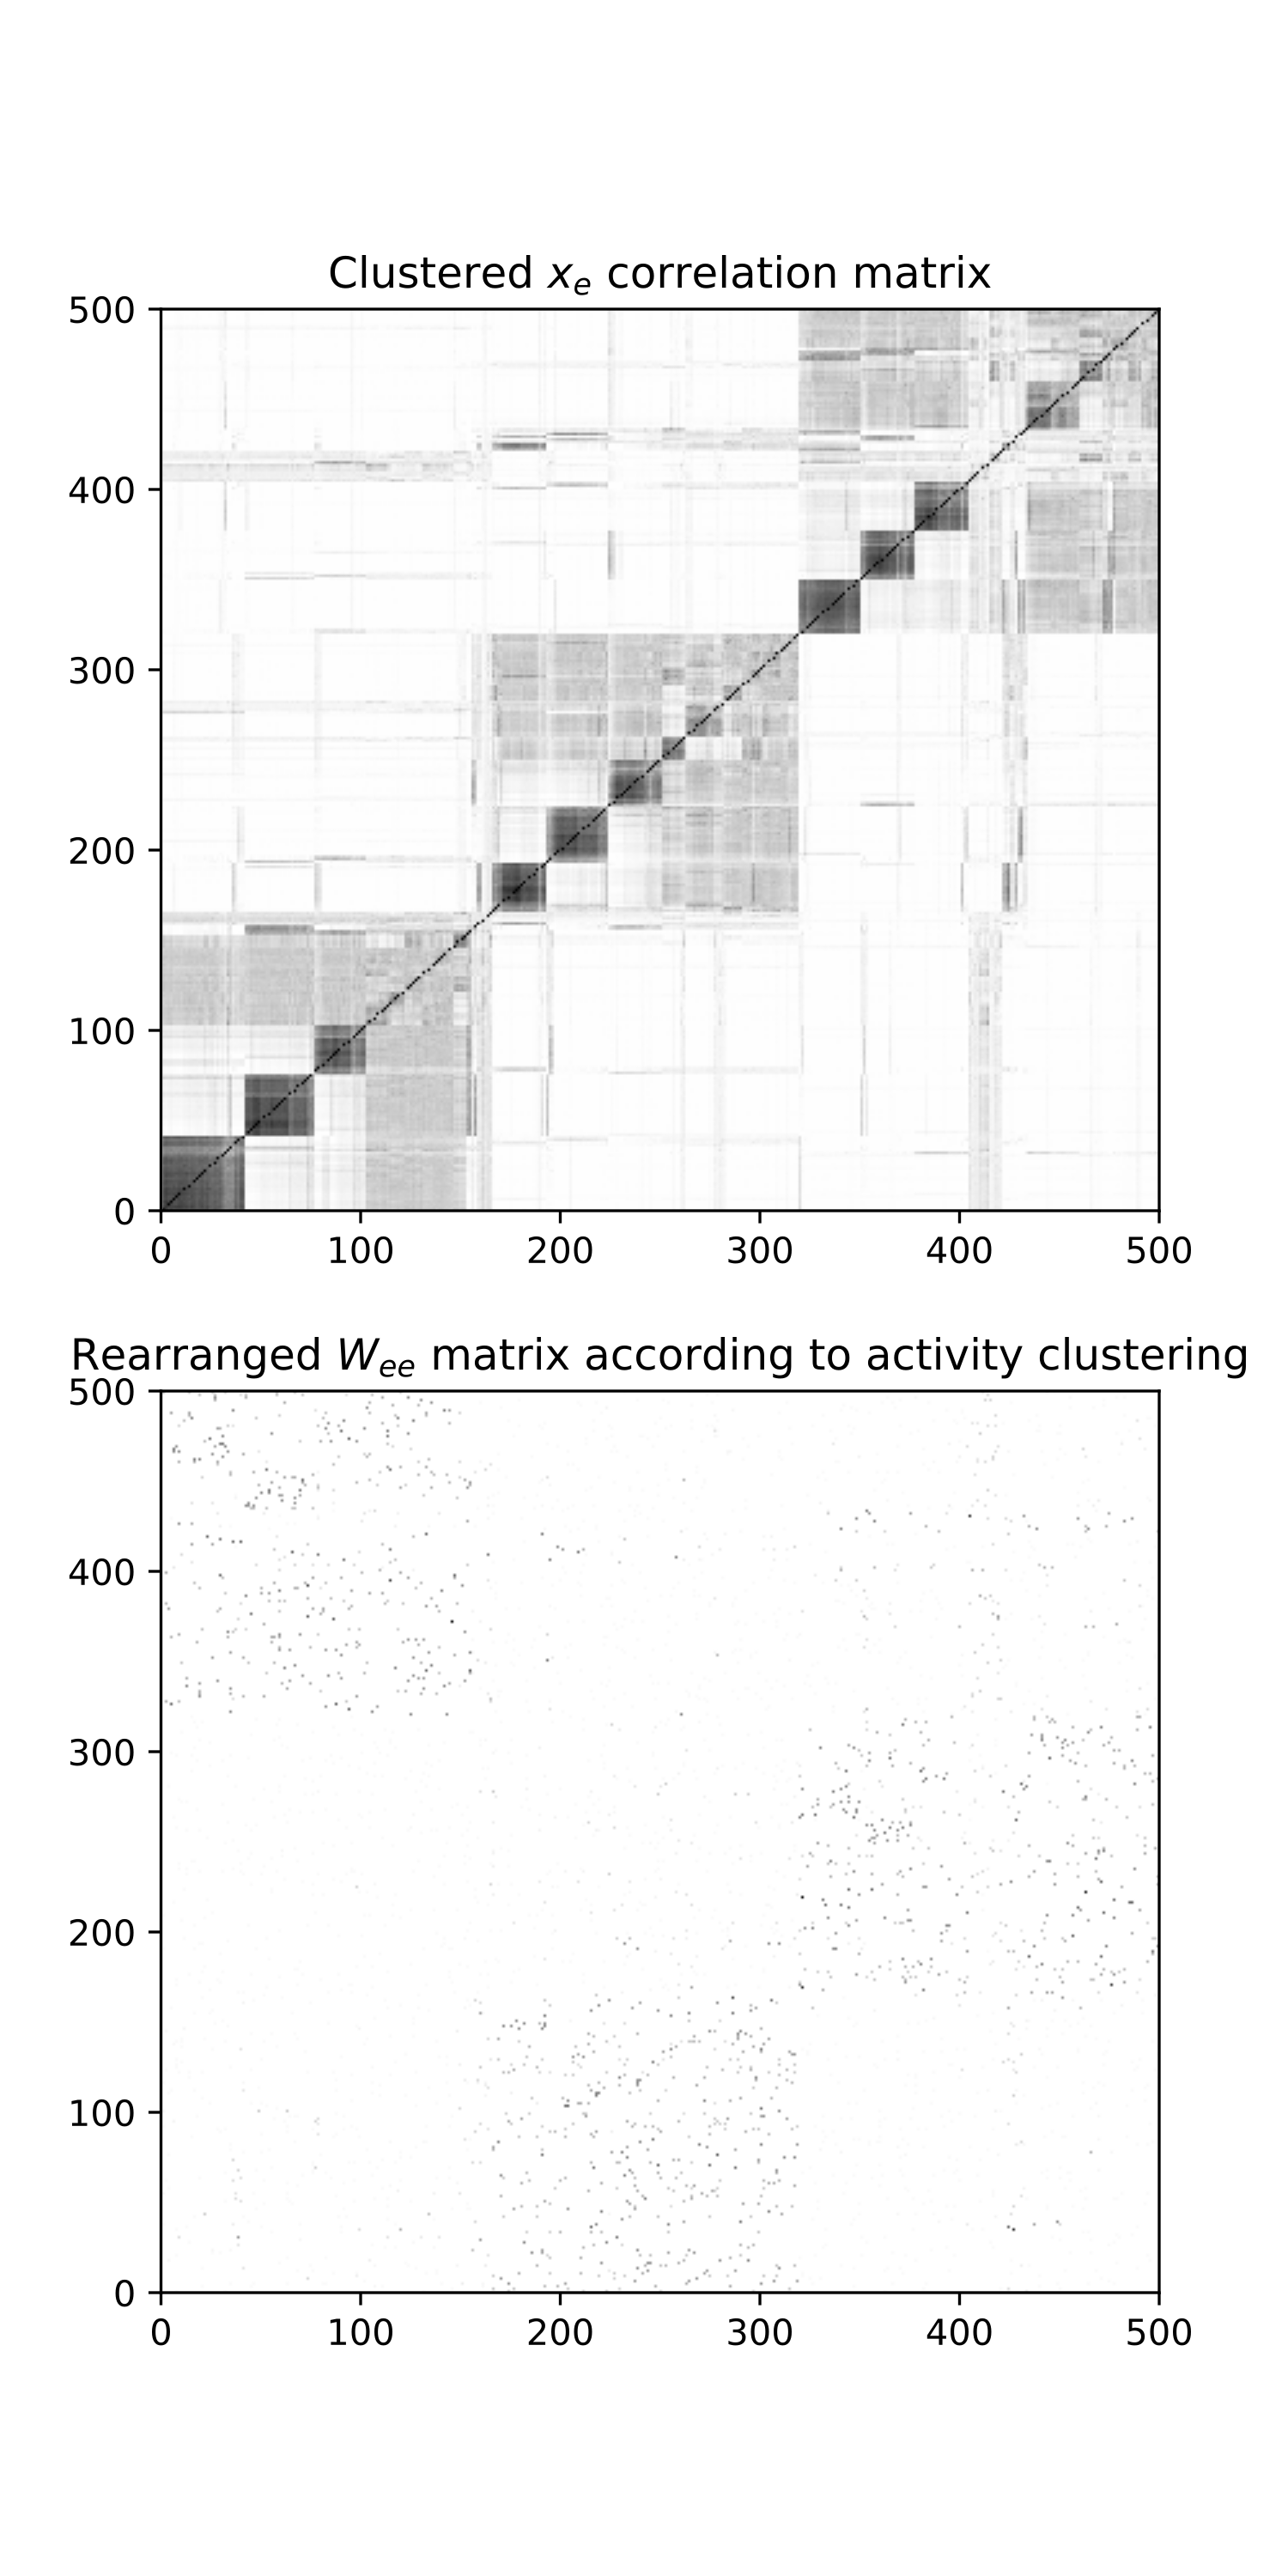
\includegraphics[width=0.8\textwidth]{../../plots/corr_weight_mat_prox_dist.png}
\caption{\label{fig:corr_weight_mat_prox_dist} Same analysis as in Fig. \ref{fig:corr_weight_mat}, but using the phenomenological compartment model described in \eqref{f_comp1}--\eqref{f_comp4}.}
\end{figure}

\subsection{A Multi Compartment Model is not Scale Invariant}

One advantage of using a simple linear superposition of inputs in combination with a theta function as a nonlinear output is the scale invariance with respect to the input, since the up-down state separatrix in the input space is simply a plane that does not change shape under a rescale of the input. This, however, is obviously not the case for the activation function shown in Fig. \ref{fig:f_comp_plot}. Under ideal working conditions, the Input should span the region depicted in this figure. However, this is not the case if we naively pass the Input into our prox-dist activation function, as can be seen in Fig. \ref{fig:prox_dist_act_cloud}.

\begin{figure}
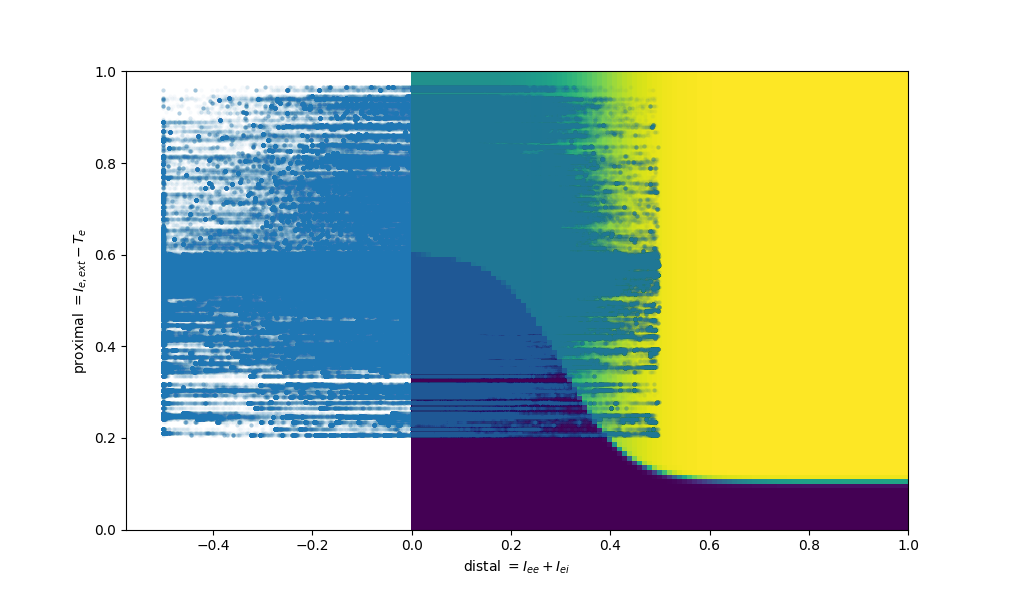
\includegraphics[width=\textwidth]{../../plots/prox_dist_act_cloud.png}
\caption{\label{fig:prox_dist_act_cloud} Overlay of proximal-distal inputs that the excitatory neurons received throughout the simulation over the activation function shown in Fig. \ref{fig:f_comp_plot}. Each blue dot represents a pair of proximal and distal input.}
\end{figure}



\section{More Complex Input Sequences}
In the input sequence used in the previous section each letter corresponds to a a particular state in a Markov model. Thus, the prediction of the next letter only requires knowledge about the previous letter received. A more realistic kind of input stream would require the network to gather information about multiple time steps in order to optimally predict the next letter. Such a kind of artificial grammar was also used in \citep{Duarte_2014} and initially introduced by Reber \cite{Reber_1967}. It is depicted in Fig. \ref{fig:Reber_Grammar}(top). Interestingly, the rules of this grammar is described as a finite-state machine where the \textit{transitions} between states correspond to letters. Of course, this kind of representation of the dynamics also has a counterpart where letters are identified with states, see the bottom network in Fig. \ref{fig:Reber_Grammar}. Our previous analysis of network activity was based on the assumption that letters, or sets of letters were represented by states of the recurrent network and not in transitions between those. In consequence, a reflection of the Reber grammar within the network should resemble the mapping shown in the bottom network of Fig. \ref{fig:Reber_Grammar}. 
\begin{figure}
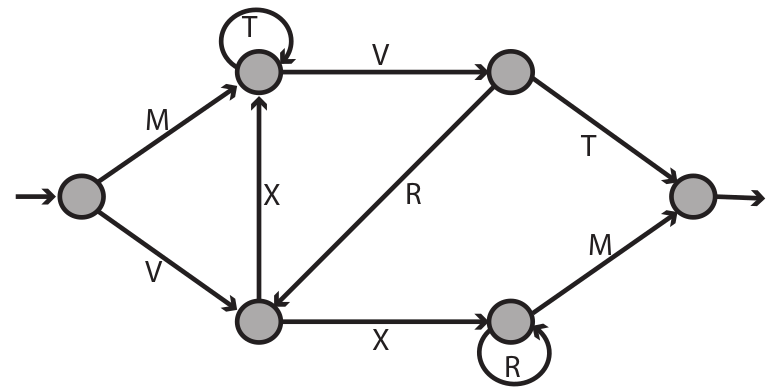
\includegraphics[width=0.7\textwidth]{../../plots/artif_grammar_illustration.png}
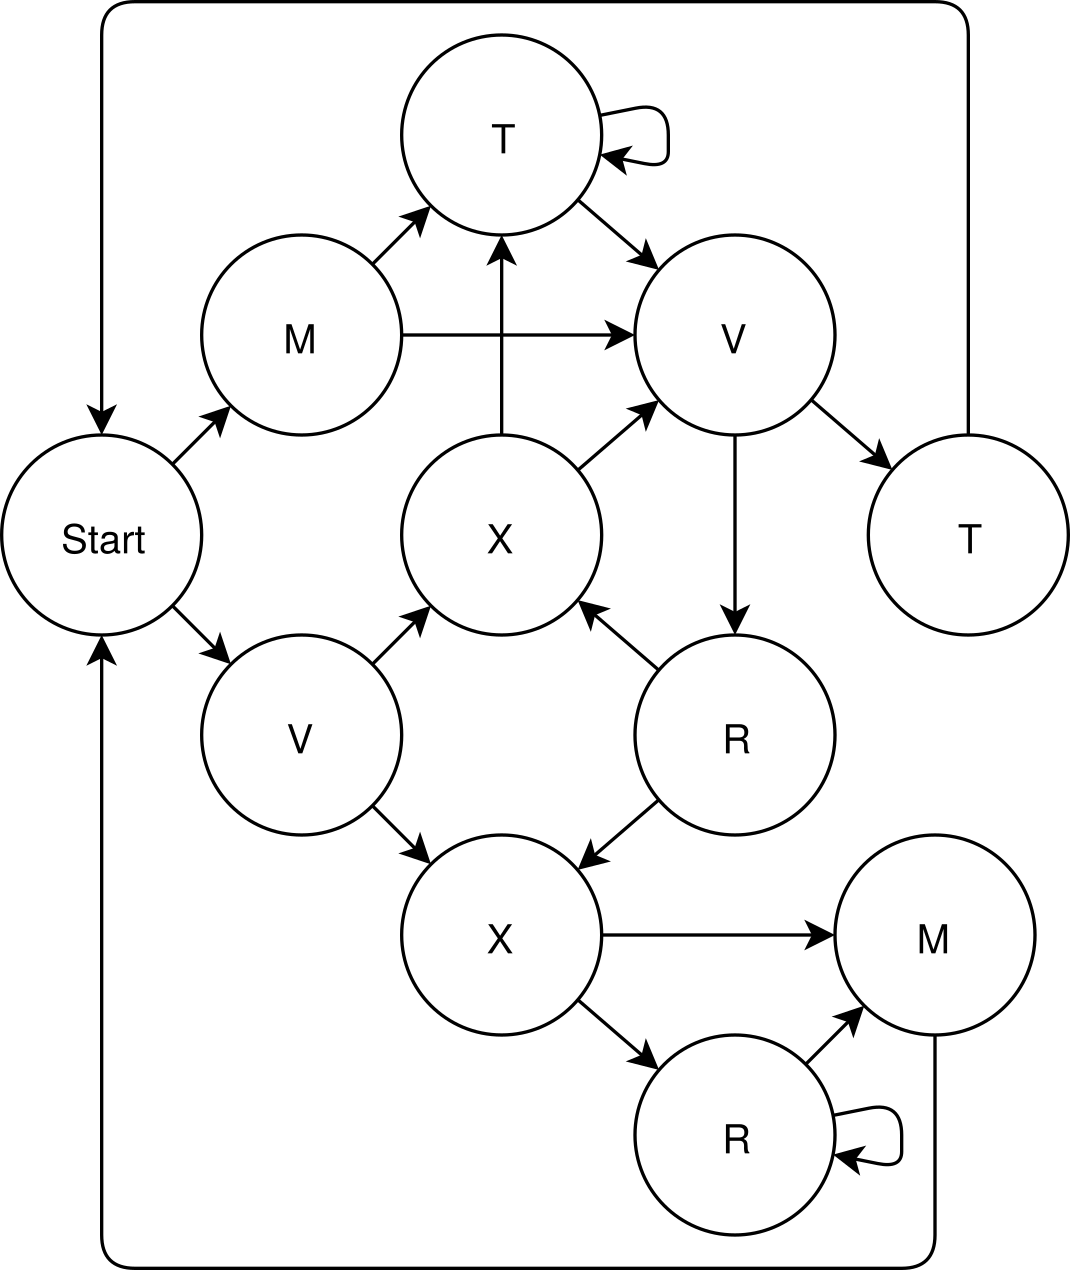
\includegraphics[width=0.5\textwidth]{../../plots/Reber_Grammar_States.png}
\caption{Artificial Grammar Rule proposed by Reber \citep{Reber_1967} (top) and the corresponding network where letters are represented by states (bottom).}
\label{fig:Reber_Grammar}
\end{figure}


\section{Using a non-binary network with plastic inputs}

Generalizing the model presented in Section \ref{Methods}, we implemented a network version, where
\begin{itemize}
\item the distinction between excitatory and inhibitory neurons was omitted. Each neuron could have both outgoing connections with both positive and negative sign.
\item The step-activation function was replaced by a continuous sigmoidal function.
\item The recurrent network had all-to-all connectivity.
\item External inputs were also initialized fully connected and subject to plasticity.
\end{itemize}

The input grammar was chosen to be the same as shown in Fig. \ref{fig:grammar_markov}. An example for the resulting activity is shown in Fig. \ref{fig:act_plot_non_bin}. After a transient phase of fluctuating activity, the recurrent network almost completely stabilizes into a combination of upper and lower activity states. Note that the fixed activity states ($0.1$ and $0.9$) correspond to the fixed points of the membrane potential in the nonlinear Hebbian learning rule. As Fig. \ref{fig:lyap_exp} illustrates, the system appears to become non-chaotic---in the sense that close-by trajectories converge---long before it enters its quasi-stable state. 

\begin{figure}
\begin{center}
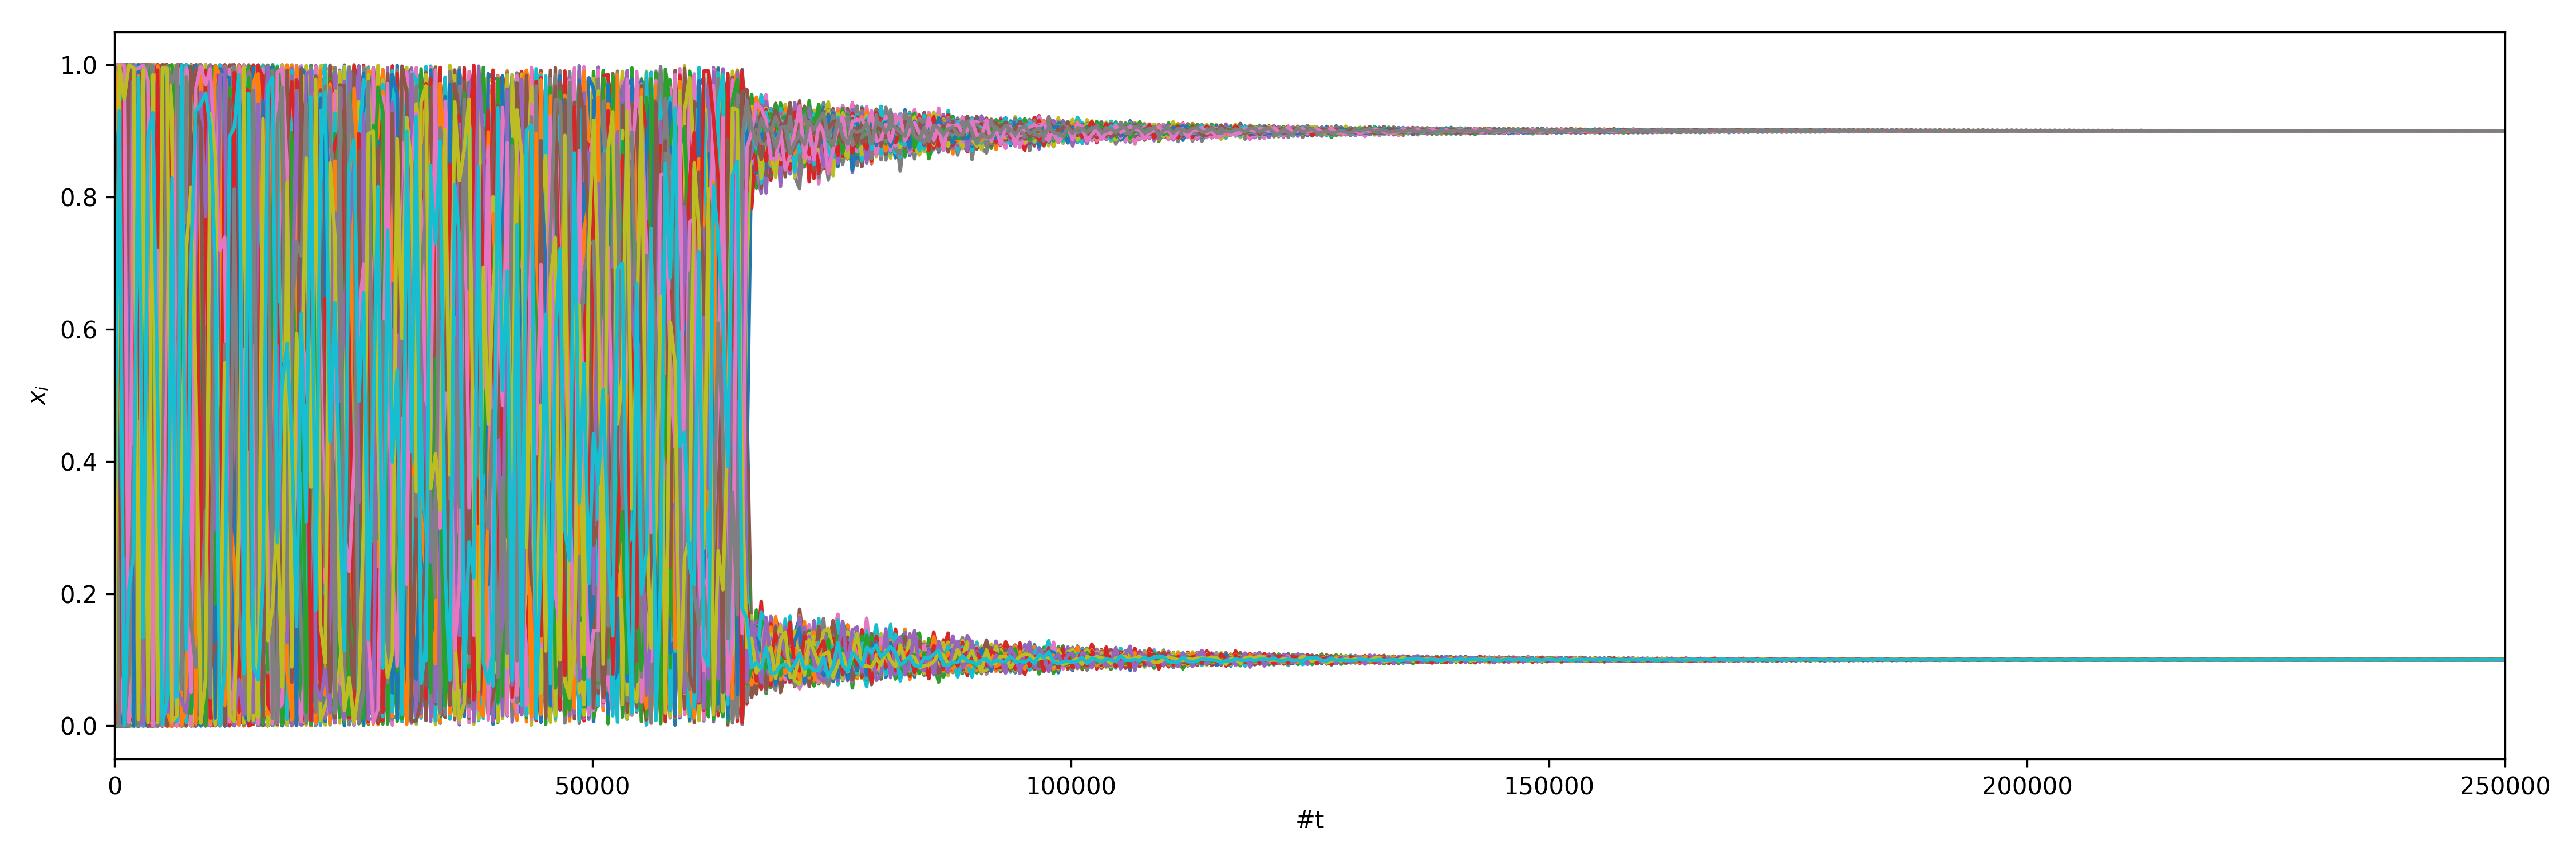
\includegraphics[width=\textwidth]{../../code/rnn_prox_dist_non_bin/plots/plastic_input_weights_small_init/activity_plot.png}
\end{center}
\label{fig:act_plot_non_bin}
\caption{Activity of recurrent non binary network.}
\end{figure}

\begin{figure}
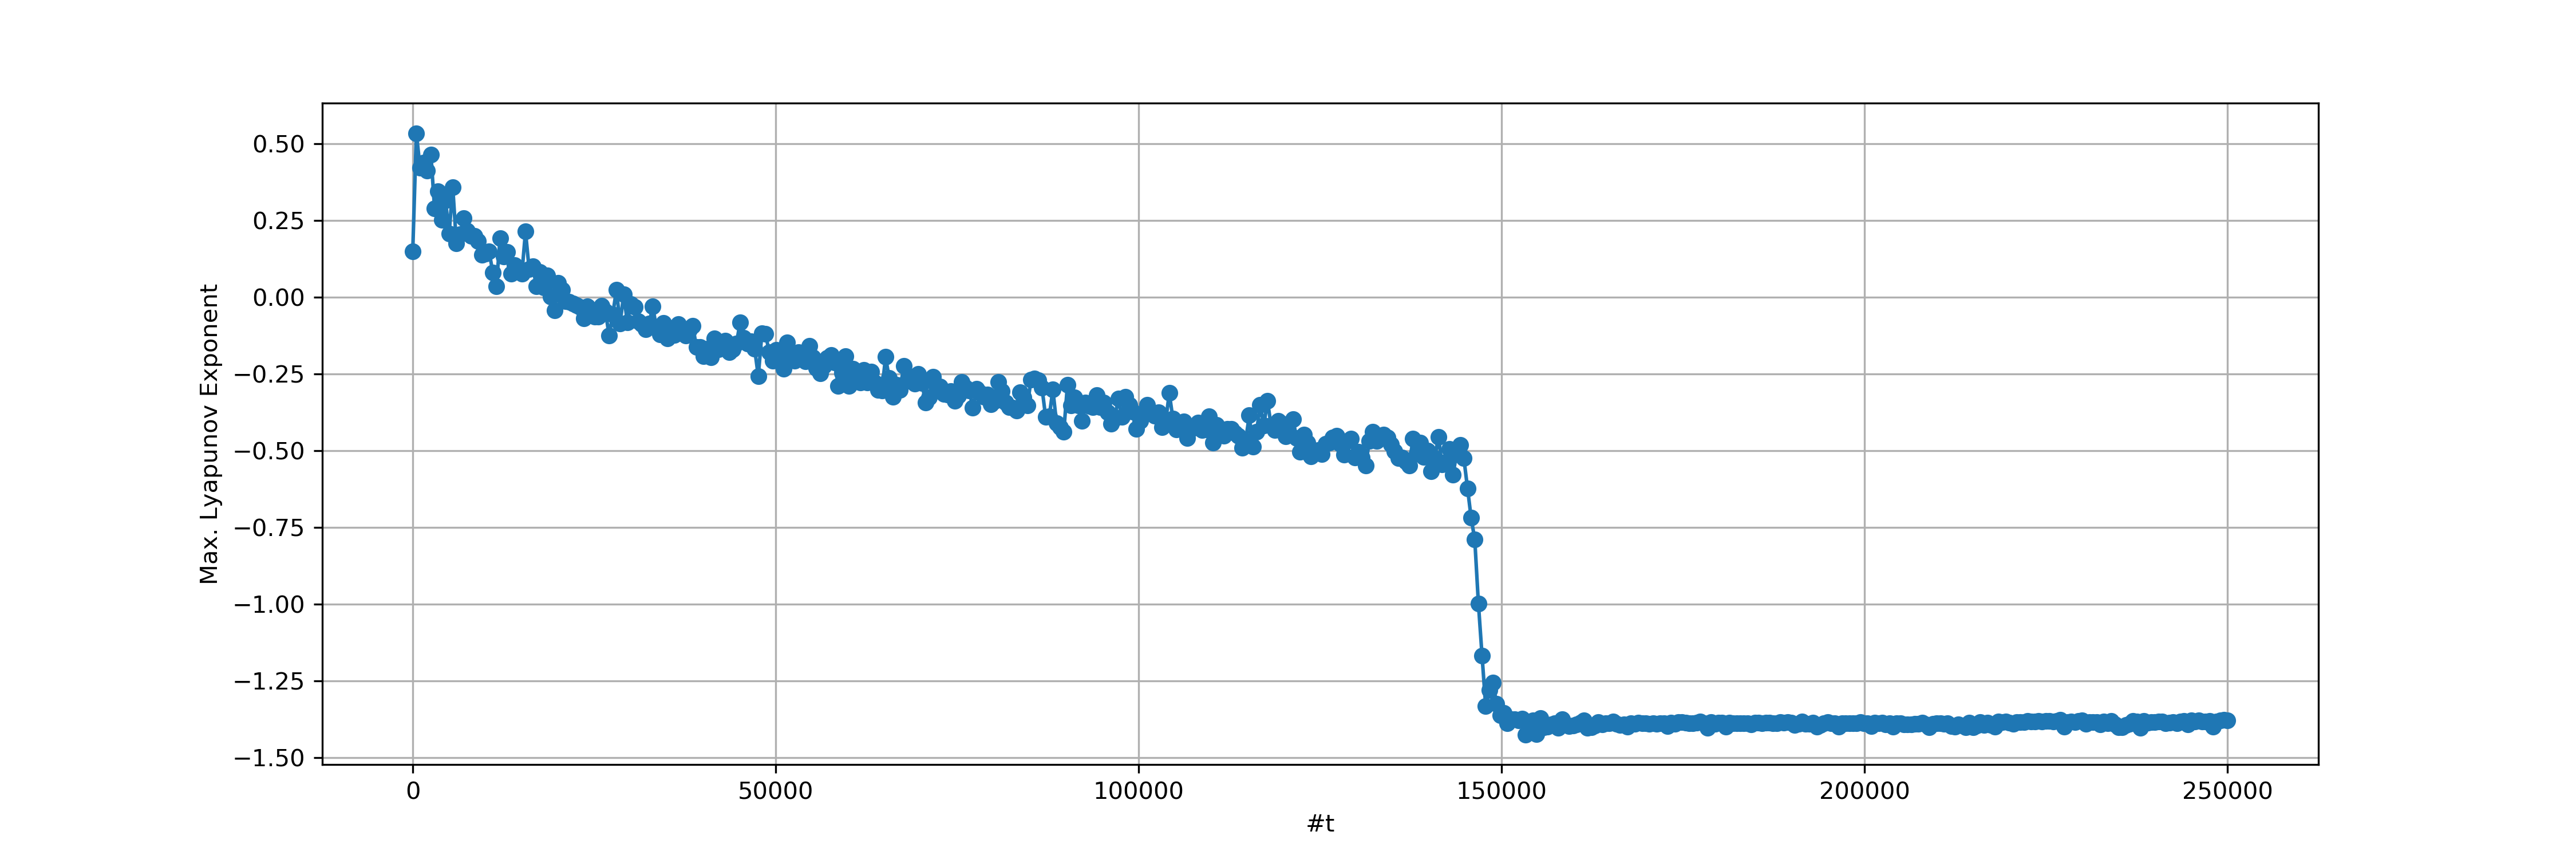
\includegraphics[width=\textwidth]{../../code/rnn_prox_dist_non_bin/plots/plastic_input_weights_small_init/lyapunov_exponents.png}
\label{fig:lyap_exp}
\caption{Largest Lyapunov exponent of the recurrent system along the trace of activity shown in Fig. \ref{fig:act_plot_non_bin}.}
\end{figure}

\subsection{Balance between recurrent and excitatory input}

Does a neuron retain a balance between the integration of external input and recurrent connections? We tested compared the dynamics of input currents throughout the simulation given two initial conditions: First, the standard deviation of external weights was initially small compared to the recurrent connections (10 times smaller). In the second case, the standard deviation of the random external weights were initialized 5 times larger than the recurrent connections. In both cases, the mean of both connection types was set to zero. As shown in Fig. \ref{fig:I_std_small_init} and \ref{fig:I_std_large_init}, both initial conditions led to a similar standard deviation of input currents until the transition to the stable network state is reached. A more detailed illustration of the evolving distribution is shown in Fig. \ref{fig:I_hist_small_init} and \ref{fig:I_hist_large_init}. Corresponding to our observation with respect to neural activity, the stable phase is characterized by a sudden splitting of recurrent input currents.

\begin{figure}
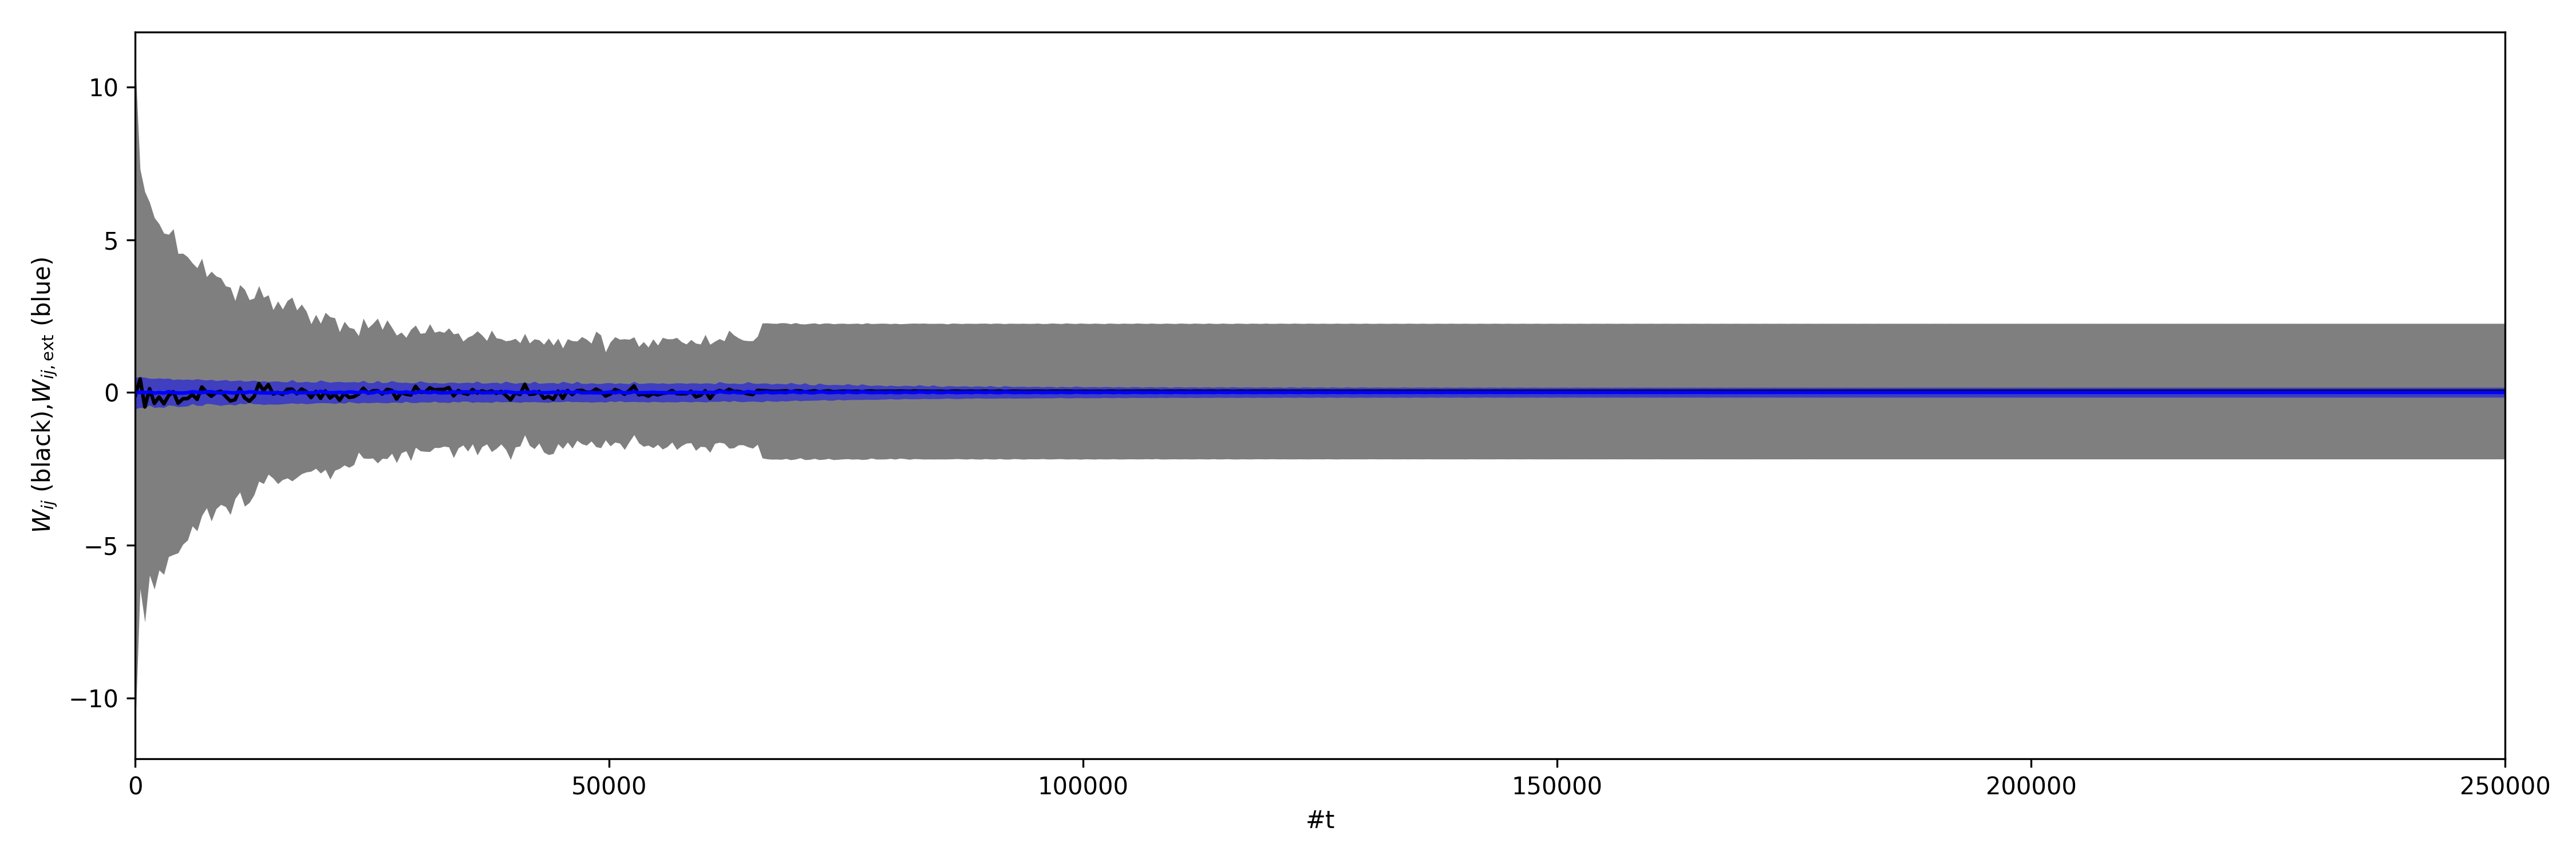
\includegraphics[width=\textwidth]{../../code/rnn_prox_dist_non_bin/plots/plastic_input_weights_small_init/I_ee_I_eext_mean_std.png}
\label{fig:I_std_small_init}
\caption{Mean and standard deviation across the population of the external and recurrent input current, small initial external connections.}
\end{figure}

\begin{figure}
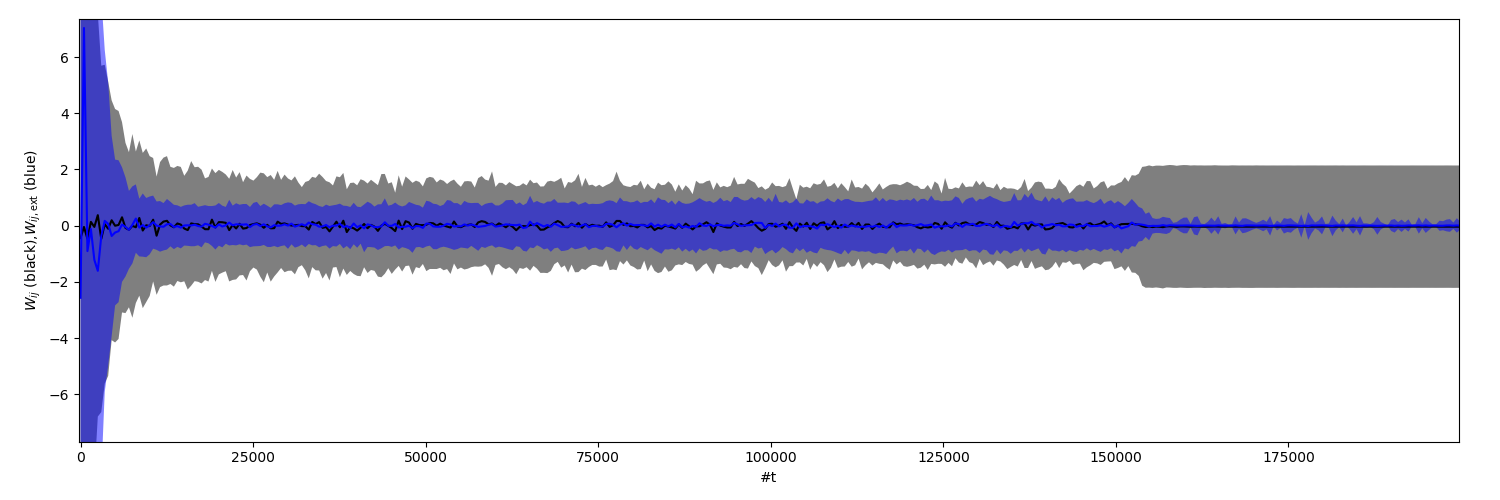
\includegraphics[width=\textwidth]{../../code/rnn_prox_dist_non_bin/plots/plastic_input_weights_large_init/I_ee_I_eext_mean_std.png}
\label{fig:I_std_large_init}
\caption{Mean and standard deviation across the population of the external and recurrent input current, large initial external connections.}
\end{figure}

\begin{figure}
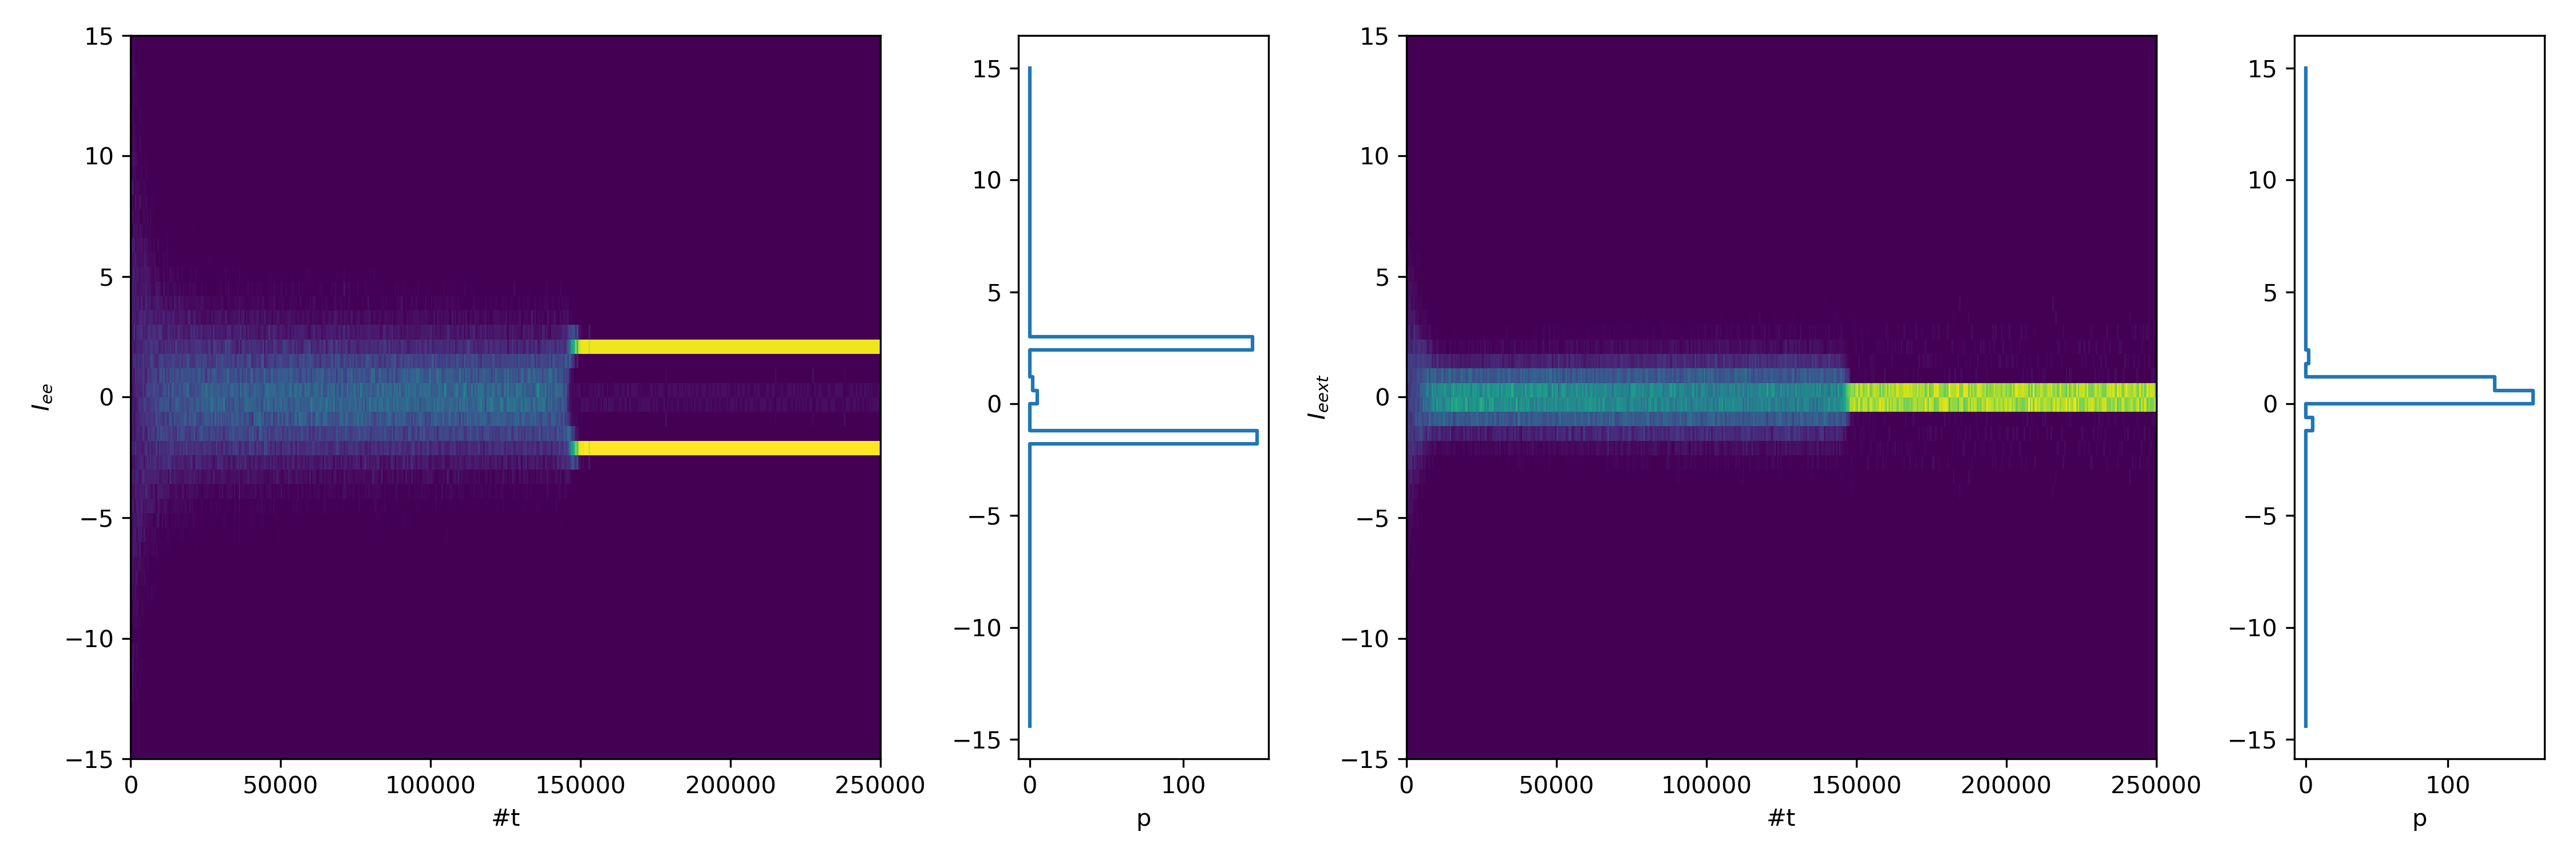
\includegraphics[width=\textwidth]{../../code/rnn_prox_dist_non_bin/plots/plastic_input_weights_small_init/input_hist_time.png}
\label{fig:I_hist_small_init}
\caption{Histogram across the population of the external and recurrent input current, small initial external connections.}
\end{figure}

\begin{figure}
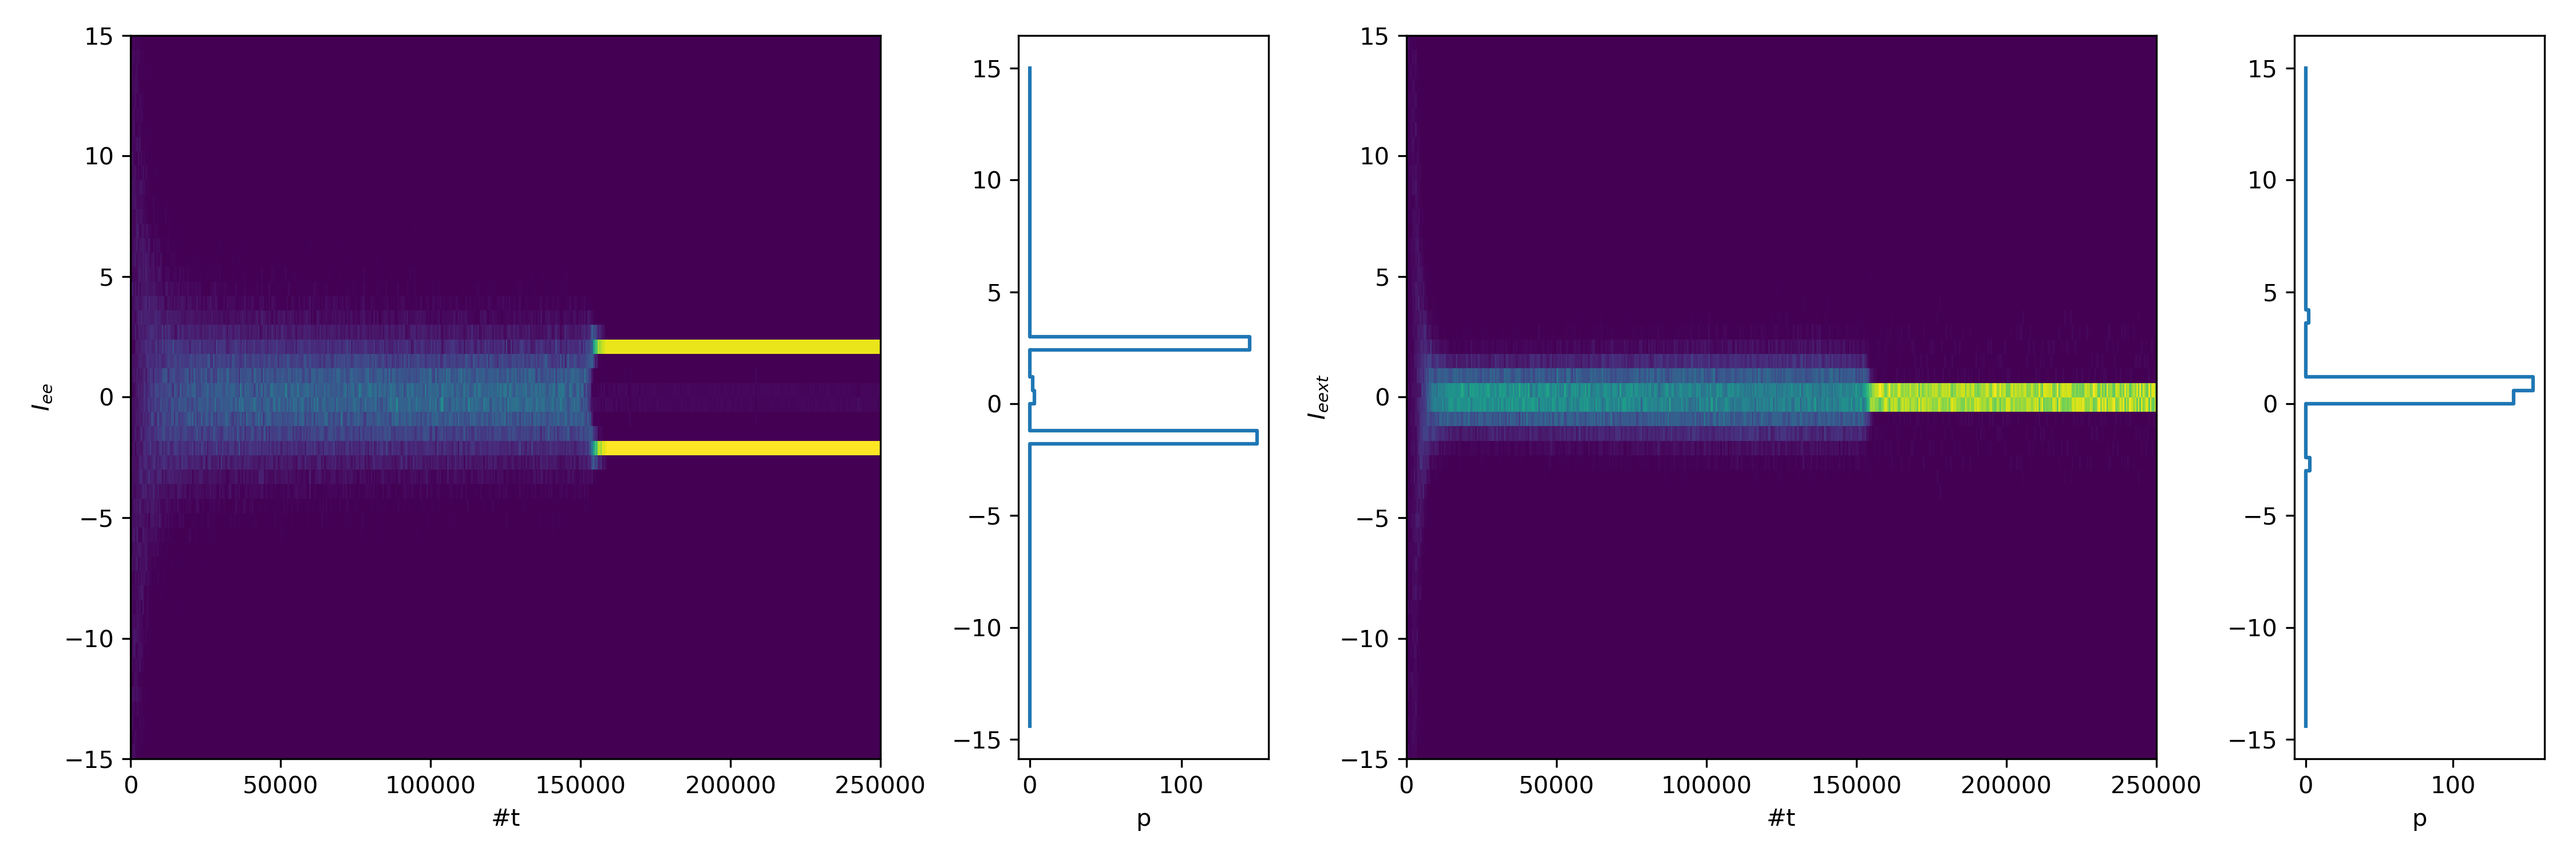
\includegraphics[width=\textwidth]{../../code/rnn_prox_dist_non_bin/plots/plastic_input_weights_large_init/input_hist_time.png}
\label{fig:I_hist_large_init}
\caption{Histogram across the population of the external and recurrent input current, large initial external connections.}
\end{figure}



\newpage
\bibliographystyle{unsrt}
\bibliography{../code/ipynb_biblio}

\end{document}